\documentclass[UTF8,a4paper,11pt]{ctexart}

\usepackage{amsmath,amssymb,bm,mathtools}
\usepackage{booktabs,array,tabularx,longtable}
\usepackage{xcolor}
\usepackage{graphicx}
\usepackage{geometry}
\usepackage{enumitem}
\usepackage{hyperref}
\usepackage{fancyhdr}
\usepackage{tcolorbox}

\geometry{left=24mm,right=24mm,top=25mm,bottom=25mm}
\hypersetup{colorlinks=true,linkcolor=blue!55!black,urlcolor=blue!55!black}
\setlength{\parindent}{2em}
\setlength{\parskip}{0.35em}
\setlength{\headheight}{14pt}
\setlist[itemize]{leftmargin=2.2em,itemsep=0.2em}
\setlist[enumerate]{leftmargin=2.4em,itemsep=0.25em}
\pagestyle{fancy}
\fancyhf{}
\fancyhead[L]{Kalman 高斯融合的矩阵含义}
\fancyhead[R]{\thepage}
\renewcommand{\headrulewidth}{0.4pt}

\newtcolorbox{keybox}{
  colback=blue!4,
  colframe=blue!55!black,
  boxrule=0.7pt,
  arc=2mm,
  left=2mm,right=2mm,top=1.5mm,bottom=1.5mm
}
\newtcolorbox{warnbox}{
  colback=orange!6,
  colframe=orange!75!black,
  boxrule=0.7pt,
  arc=2mm,
  left=2mm,right=2mm,top=1.5mm,bottom=1.5mm
}

\newcommand{\prior}{^{-}}
\newcommand{\transpose}{^{\mathsf T}}

\title{从单个高斯分布到 Kalman 矩阵融合\\
\large 以状态 $[x,y,v]\transpose$ 为例解释每个元素如何修正状态与协方差}
\author{Kalman 编队算法数学说明}
\date{2026 年 11 月}

\begin{document}
\maketitle
\tableofcontents
\newpage

\section*{引言与阅读导图}
\addcontentsline{toc}{section}{引言与阅读导图}

本文并非按照传统教材中“先给出 Kalman 公式，再解释公式用途”的顺序写成，而是起源于一个具体的编队跟踪问题：当领导者的位置观测含有噪声时，如何利用运动模型和位置测量估计其当前状态，并把估计结果可靠地传递给后续虚拟载具与跟踪控制器？围绕这一问题，程序经历了“加入噪声与滤波---观察仿真结果---提出数学疑问---展开矩阵推导---返回程序验证”的多轮修改。本文保留了这一认识过程，希望回答的不只是“Kalman 滤波公式怎样使用”，还包括“每个矩阵究竟描述什么概率对象”“矩阵中的单个元素如何影响状态修正”以及“理论上完整的协方差模型是否一定更适合当前程序”。

第 1 节首先回答滤波器所服务的对象如何运动。领导者采用非完整约束移动机器人的圆弧运动学模型，状态估计量选为 $[x,y,v]^{\mathsf T}$，航向角 $\theta$ 和角速度 $w$ 则作为已知运动学输入直接传递。这样既说明了位置和速度如何由上一时刻传播到下一时刻，也确定了后续协方差传播矩阵 $F_k$ 的来源。第 2 节进一步回答“为什么一个实际位置可以用高斯分布表示”以及“两个高斯分布怎样融合”：真实位置本身并不是分布，高斯分布描述的是估计器对未知真实位置的认识；先验分布与测量似然相乘后，得到后验方差
\begin{equation}
P=\left[(P\prior)^{-1}+R^{-1}\right]^{-1}
=\frac{P\prior R}{P\prior+R},
\end{equation}
以及后验均值
\begin{equation}
\mu=\mu\prior+K(z-\mu\prior),
\qquad
K=\frac{P\prior}{P\prior+R}.
\end{equation}
这一节建立全文最基础的直觉：Kalman 滤波的测量更新，本质上仍然是高斯概率信息的融合。

从第 3 节开始，问题由单变量融合扩展到多维矩阵计算。第 3 节分别定义状态先验分布、理想预测测量、测量噪声、创新分布、状态--测量交叉协方差和后验分布，重点区分创新协方差
\begin{equation}
S_k=HP_k\prior H\transpose+R
\end{equation}
与融合后的后验协方差 $P_k$。前者描述“实际测量与先验预测测量之差可能波动多大”，后者才描述融合后状态分布还剩多少不确定性。第 4 节接着回答“矩阵 Kalman 增益如何把位置残差变成 $x,y,v$ 三个状态量的修正量”，说明
\begin{equation}
K_k=P_k\prior H\transpose S_k^{-1}
\end{equation}
既包含各测量方向的可信程度，也包含测量误差与各状态误差之间的关联。第 5 节通过一个可以逐项手算的 $[x,v]^{\mathsf T}$ 示例，把先验状态、真实状态、测量噪声、创新、Kalman 增益和状态修正量全部代入具体数值，从而说明 $K_k\bm r_k$ 是后验均值相对于先验均值的修正量，而不是后验误差本身。

第 6 节集中回答全文推导中最容易产生混淆的问题：后验协方差究竟怎样由后验误差得到，以及测量噪声是否在最优滤波后被“归零”。该节从先验误差、测量方程和状态更新方程开始，不跳步地推导
\begin{equation}
\bm e_k=(I-K_kH)\bm e_k\prior-K_k\bm\nu_k,
\end{equation}
再对误差外积取期望，得到 Joseph 协方差公式
\begin{equation}
P_k
=(I-K_kH)P_k\prior(I-K_kH)\transpose
+K_kRK_k\transpose.
\end{equation}
第一项表示先验误差经过测量修正后剩余的部分，第二项表示测量噪声经 Kalman 增益传入后验估计的部分。因此，最优 Kalman 增益并没有令噪声消失，而是在先验不确定性与测量噪声之间选择使后验协方差最小的权重。

第 7 节重新回到“两个高斯分布相乘”的视角，将标量高斯融合与 Joseph 矩阵递推连接起来，并解释为什么
\begin{equation}
K_k=P_k\prior H\transpose S_k^{-1}
\end{equation}
和
\begin{equation}
K_k=P_kH\transpose R^{-1}
\end{equation}
都是正确的计算关系，只是采用了不同的计算路线。该节还专门比较创新协方差 $S_k$ 与后验协方差 $P_k$：$S_k$ 是求解增益时使用的中间概率量，$P_k$ 才是决定后验高斯分布宽度并继续进入下一次递推的融合协方差。

第 8 节回答“过程噪声 $Q_k$ 从哪里来”。$Q_k$ 不是下一时刻实际误差，也不是先验状态与后验状态之差，而是用来描述加速度变化、打滑、执行器偏差和模型不完整性在一次运动传播中新增的不确定性。它通过
\begin{equation}
P_{k+1}\prior=F_kP_kF_k\transpose+Q_k
\end{equation}
与原有后验不确定性共同形成下一时刻的先验协方差。第 9 节则把此前分散讨论的概率对象、均值更新和协方差更新重新排列为一次完整递推，给出“后验---运动传播---先验---观测---创新---增益---新后验”的因果顺序，并分别总结 Kalman 增益、最优状态估计、融合协方差和过程噪声之间的关系。

第 10 节把理论进一步带回当前 MATLAB 程序，回答 $p_{xv}$、$p_{yv}$ 和 $p_{xy}$ 如何由运动模型产生，以及它们分别如何进入 Kalman 增益。由
\begin{equation}
P_{k+1}\prior=F_kP_kF_k\transpose+Q_k
\end{equation}
可知，同一个速度误差在传播过程中会同时影响 $x$ 和 $y$，从而自然形成位置--速度协方差及位置间交叉协方差。其中，$p_{xv}$ 和 $p_{yv}$ 决定位置创新能否修正速度，$p_{xy}$ 则决定两个位置创新应当如何联合解释。为了判断这种理论上的耦合是否适合当前模型，程序又进行了完整协方差与强制 $p_{xy}=0$ 的对照实验。在相同随机种子、噪声序列和参数下，强制 $p_{xy}=0$ 后，先验位置 RMSE 由 $0.033276\,\mathrm m$ 降至 $0.025262\,\mathrm m$，后验位置 RMSE 由 $0.031789\,\mathrm m$ 降至 $0.023382\,\mathrm m$。这一结果说明：交叉协方差在一般联合高斯模型中具有严格意义，但当当前程序的 $x,y$ 观测被独立建模时，不准确或不必要的耦合也可能把一个方向的噪声传播到另一个方向。该结论目前只适用于这一轨迹、随机种子和参数组合，不能推广为所有 Kalman 滤波器都应删除 $p_{xy}$。

最后，第 11 节建立数学符号与 MATLAB 变量之间的逐项映射。主要变量 \nolinkurl{prior_state}、\nolinkurl{innovation_covariance}、\nolinkurl{kalman_gain}、\nolinkurl{posterior_state} 和 \nolinkurl{posterior_covariance} 分别对应 $\hat{\bm x}_k\prior$、$S_k$、$K_k$、$\hat{\bm x}_k$ 和 $P_k$。因此，读者既可以从前向后理解完整的概率与矩阵推导，也可以从程序中的某个变量反向查找其概率含义、计算来源和对后续状态更新的作用。

整体阅读路线可以概括为
\begin{equation}
\boxed{
\begin{gathered}
\text{载具怎样运动}
\longrightarrow
\text{两个高斯怎样融合}
\longrightarrow
\text{标量怎样推广为矩阵}\\
\longrightarrow
\text{增益怎样修正状态}
\longrightarrow
\text{协方差怎样递推}
\longrightarrow
\text{程序实验是否支持该模型}.
\end{gathered}
}
\end{equation}
文中的公式推导、数值代入和 $p_{xy}=0$ 对照实验并不是互相独立的材料，而是对同一个状态估计问题逐层深入后形成的三类证据。

\newpage

\section{智能体的运动学模型}

本文的领导者和虚拟载具采用非完整约束移动机器人的运动学模型。智能体位姿为
\begin{equation}
\bm q(t)=
\begin{bmatrix}
x(t)&y(t)&\theta(t)
\end{bmatrix}\transpose,
\end{equation}
其中 $x,y$ 是世界坐标系中的位置，$\theta$ 是航向角。纵向线速度为 $v$，角速度为 $w$，连续时间运动学方程为
\begin{align}
\dot x(t)&=v(t)\cos\theta(t),\\
\dot y(t)&=v(t)\sin\theta(t),\\
\dot\theta(t)&=w(t).
\end{align}

当一个采样周期 $\Delta t$ 内的 $v_k,w_k$ 近似保持不变，且 $w_k\neq0$ 时，对上式积分得到同构圆弧传播模型
\begin{align}
x_{k+1}
&=x_k+
\frac{v_k}{w_k}
\left[
\sin(\theta_k+w_k\Delta t)-\sin\theta_k
\right],\\
y_{k+1}
&=y_k+
\frac{v_k}{w_k}
\left[
\cos\theta_k-\cos(\theta_k+w_k\Delta t)
\right],\\
\theta_{k+1}&=\theta_k+w_k\Delta t.
\end{align}

当 $w_k$ 接近零时，上式的极限为直线传播模型
\begin{align}
x_{k+1}&=x_k+v_k\cos\theta_k\,\Delta t,\\
y_{k+1}&=y_k+v_k\sin\theta_k\,\Delta t,\\
\theta_{k+1}&=\theta_k.
\end{align}

当前 Kalman 滤波器递归估计的状态选为
\begin{equation}
\bm x_k=
\begin{bmatrix}
x_k&y_k&v_k
\end{bmatrix}\transpose.
\end{equation}
航向角 $\theta_k$ 和角速度 $w_k$ 不进入 Kalman 状态，而是作为已知运动学输入直接传递。这样既保留了与真实载具同构的圆弧运动模型，也避免航向角滤波超调直接作用于编队控制器。真实车辆中若 $\theta_k,w_k$ 本身含有噪声，则仍需通过过程噪声协方差 $Q_k$ 或独立航向估计器描述其影响。

\section{位置的高斯概率模型与基础高斯融合}

\subsection{为什么用高斯分布表示位置}

载具在某一时刻只有一个真实位置 $x_k^{\mathrm{true}}$，真实位置本身不是一团高斯分布。高斯分布描述的是：在真实位置未知的情况下，估计器对位置可能取值及其不确定性的认识。

位置测量会受到传感器噪声、采样误差和模型误差影响。当大量相互独立的小误差共同作用时，合成误差通常可以近似为高斯分布。因此，可以用
\begin{equation}
x\sim\mathcal N(\mu,\sigma^2)
\end{equation}
表示对位置 $x$ 的估计。其中 $\mu$ 是位置估计的中心，$\sigma^2$ 是位置估计误差的方差；方差越小，分布越窄，对位置越确定；方差越大，分布越宽，对位置越不确定。

假设运动模型给出的先验位置为
\begin{equation}
x\sim\mathcal N(\mu\prior,P\prior),
\end{equation}
其中 $\mu\prior$ 是先验位置均值，$P\prior$ 是先验位置误差方差。传感器给出测量值 $z$，并假设测量噪声满足
\begin{equation}
\nu\sim\mathcal N(0,R),
\qquad
z=x+\nu.
\end{equation}
那么这次测量对真实位置提供的测量似然可以写成
\begin{equation}
p(z\mid x)
\propto
\exp\!\left[-\frac{(z-x)^2}{2R}\right],
\end{equation}
其中 $R$ 是测量噪声方差。

\subsection{两个高斯分布怎样融合}

根据 Bayes 公式，先验分布与测量似然相乘：
\begin{equation}
p(x\mid z)\propto p(z\mid x)p(x).
\end{equation}
由于二者都是高斯形式，融合后的后验分布仍然是高斯分布：
\begin{equation}
x\mid z\sim\mathcal N(\mu,P).
\end{equation}
后验方差满足
\begin{equation}
\boxed{
P=\left[(P\prior)^{-1}+R^{-1}\right]^{-1}
=\frac{P\prior R}{P\prior+R}
}.
\end{equation}
等价地，两个信息来源的精度相加：
\begin{equation}
\frac{1}{P}=\frac{1}{P\prior}+\frac{1}{R}.
\end{equation}
因此，融合后的后验方差 $P$ 小于 $P\prior$ 和 $R$，后验分布比两个输入分布都更窄。

后验均值为
\begin{equation}
\boxed{
\mu
=P\left(
\frac{\mu\prior}{P\prior}
+\frac{z}{R}
\right)
}.
\end{equation}
定义融合权重
\begin{equation}
\boxed{
K=\frac{P\prior}{P\prior+R}
},
\end{equation}
则后验均值还可以写成
\begin{equation}
\boxed{
\mu=\mu\prior+K(z-\mu\prior)
}.
\end{equation}
其中 $z-\mu\prior$ 是测量值与先验均值之差，$K$ 决定使用多少测量信息，$K(z-\mu\prior)$ 是先验均值向测量值方向移动的修正量，$P$ 则表示融合后还剩多少位置不确定性。

\begin{figure}[htbp]
\centering
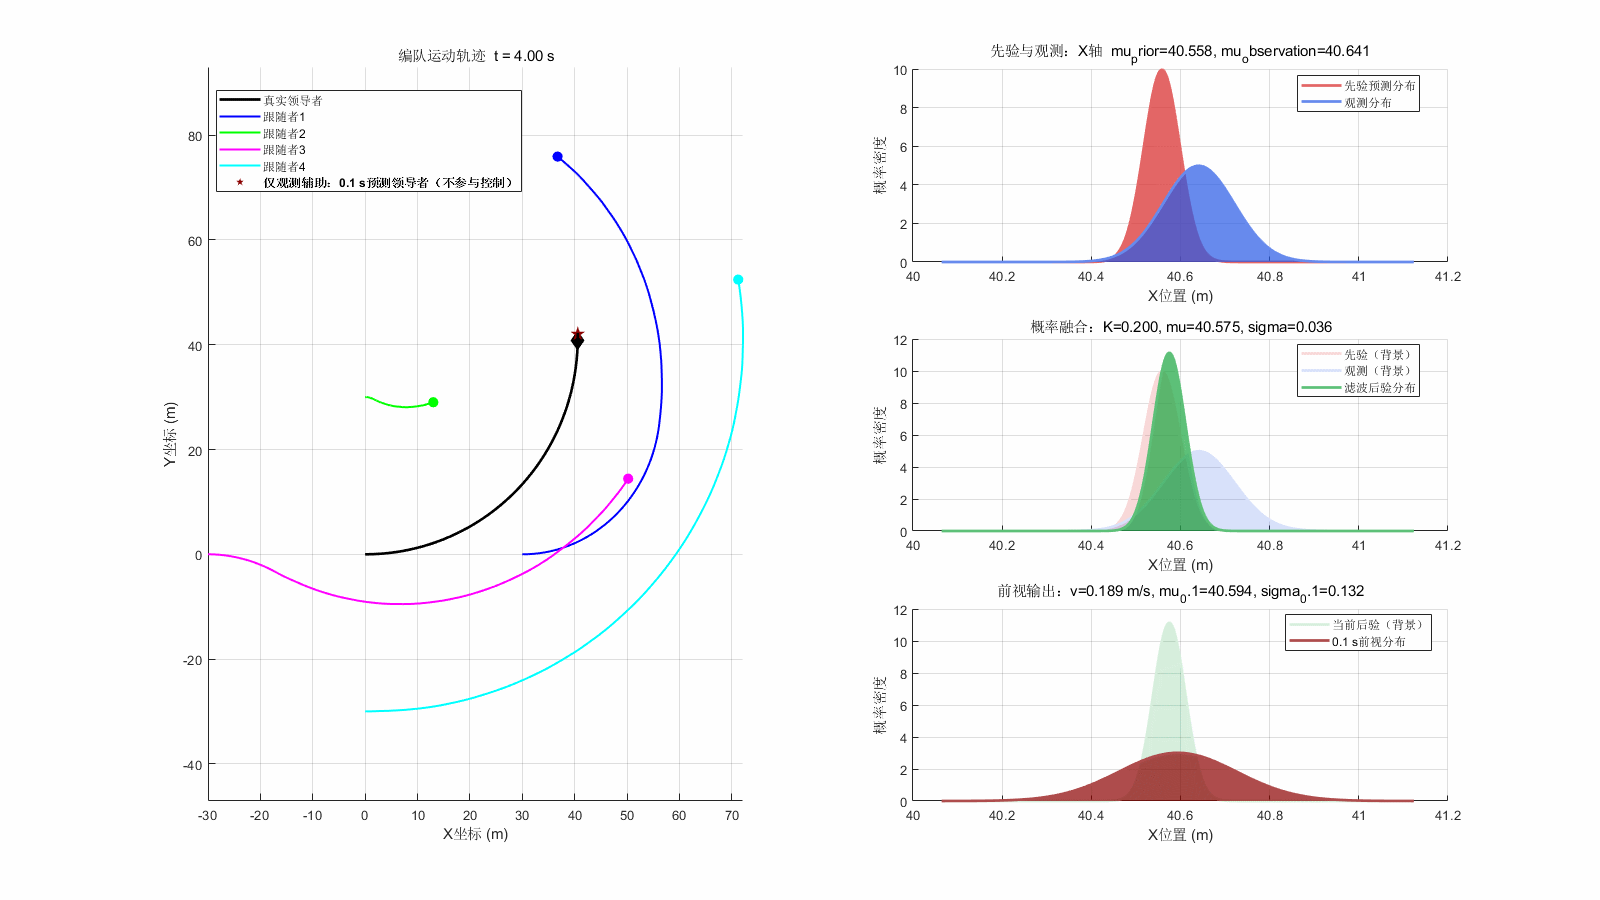
\includegraphics[width=0.98\textwidth]{assets/kalman_probability_fusion_frame_t4.png}
\caption{某一仿真时刻的 Kalman 概率融合过程。右上为先验分布与观测分布，右中绿色曲线为二者融合得到的后验分布，右下为后验状态经过运动模型传播形成的前视预测分布。}
\label{fig:kalman-fusion-frame-t4}
\end{figure}

图~\ref{fig:kalman-fusion-frame-t4} 右上给出先验位置分布与带噪声观测分布，右中给出二者融合得到的后验位置分布。右下进一步展示后验分布经过运动模型传播后形成的前视预测分布；该预测步骤不属于本节讨论的单次高斯融合，将在后续 Kalman 递推部分详细说明。

本节只描述一次高斯融合，尚未涉及时间递归。Kalman 滤波在此基础上增加运动预测，并把每一次得到的后验分布继续传递到下一时刻。

\subsection{从复习用直觉表述到严格数学定义}

\begin{keybox}
\textbf{复习用原始表述：}

单位的卡尔曼滤波，就是对多维信息来源的正态分布，基于高斯融合求解后验方差（矩阵计算就是求 Kalman 增益），执行递归算法的自适应控制器。
\end{keybox}

上面的说法保留了“高斯融合、矩阵增益、误差反馈和递归更新”四个核心直觉。若进一步修正“控制器”和“矩阵计算”的边界，可以写成：

\begin{keybox}
\textbf{直觉修订表述：}

Kalman 滤波器可以直观地理解为：把单维高斯融合推广到多维信息来源，用协方差矩阵描述各状态误差及其关联，通过矩阵运算求得 Kalman 增益，并把“测量值与先验预测值之差”作为估计误差的负反馈修正量，递归更新状态估计的状态估计负反馈修正系统。
\end{keybox}

这里的负反馈对象是状态估计误差。滤波器直接修正估计状态；只有当后续控制器使用该估计状态时，它才会间接影响载具的跟踪误差。因此，“状态估计负反馈修正系统”比“自适应控制器”更准确。

\begin{keybox}
\textbf{严格数学表述：}

Kalman 滤波器是一种面向动态系统的递归 Bayes 状态估计器：它用多元高斯分布表示先验状态与测量的不确定性，通过矩阵形式的高斯融合计算 Kalman 增益，并递归更新后验均值与后验协方差。
\end{keybox}

由于 Kalman 增益会随先验协方差和测量噪声协方差自动变化，滤波器能够自适应地调整预测信息与测量信息的融合权重；但这种“自适应”是估计权重的自适应，不代表 Kalman 滤波器本身是控制器。

一维高斯融合使用标量方差 $P\prior,R$ 和标量融合权重 $K$；推广到多维状态后，标量方差变成协方差矩阵，标量融合权重变成 Kalman 增益矩阵。因此可以说“矩阵运算的核心任务之一是求 Kalman 增益”，但不能把全部矩阵计算只等同于求增益：矩阵还要传播先验协方差，并更新融合后的后验协方差。更完整的说法是：Kalman 增益是多维高斯融合的最优权重矩阵；协方差矩阵运算则负责计算、传播和更新该权重及其不确定性依据。

\section{全部相关高斯分布及其矩阵表示}

在一次更新中，应区分下面五个对象。

\subsection{状态先验分布}
\begin{equation}
\bm x_k\sim\mathcal N(\hat{\bm x}_k\prior,P_k\prior).
\end{equation}
它存在于状态空间，本项目中维数为 3。
对应的状态协方差矩阵为
\begin{equation}
P_k\prior=
\begin{bmatrix}
p_{xx}&p_{xy}&p_{xv}\\
p_{xy}&p_{yy}&p_{yv}\\
p_{xv}&p_{yv}&p_{vv}
\end{bmatrix}.
\label{eq:state-covariance}
\end{equation}

\subsection{理想测量预测分布}

测量矩阵为
\begin{equation}
H=
\begin{bmatrix}
1&0&0\\
0&1&0
\end{bmatrix}.
\label{eq:H}
\end{equation}
它把状态映射成传感器能够看到的量：
\begin{equation}
H\bm x_k=
\begin{bmatrix}x_k\\y_k\end{bmatrix}.
\end{equation}

矩阵元素 $h_{ji}$ 的含义是：“第 $i$ 个状态量以多大系数进入第 $j$ 个测量量”。式\eqref{eq:H} 中，第一行挑选 $x$，第二行挑选 $y$，第三列为零表示传感器不直接测量 $v$。

将状态先验投影到测量空间后：
\begin{equation}
H\bm x_k\sim
\mathcal N(H\hat{\bm x}_k\prior,HP_k\prior H\transpose).
\end{equation}

对式\eqref{eq:state-covariance}执行该投影，得到
\begin{equation}
HP_k\prior H\transpose=
\begin{bmatrix}
p_{xx}&p_{xy}\\
p_{xy}&p_{yy}
\end{bmatrix}.
\end{equation}
这不是创造新方差，而是从三维状态协方差中抽取传感器可见的二维部分。

\subsection{测量噪声分布}

真实测量模型是
\begin{equation}
\bm z_k=H\bm x_k+\bm\nu_k,
\qquad
\bm\nu_k\sim\mathcal N(\bm0,R).
\end{equation}

若 $x$、$y$ 测量噪声相互独立，则
\begin{equation}
R=
\begin{bmatrix}
r_x&0\\
0&r_y
\end{bmatrix}
=
\begin{bmatrix}
\sigma_{x,\mathrm{obs}}^2&0\\
0&\sigma_{y,\mathrm{obs}}^2
\end{bmatrix}.
\end{equation}

$R$ 是测量误差协方差，不是状态预测协方差。它由传感器噪声模型、标定实验或人为调参给出。

\subsection{创新分布}

实际测量与预测测量之差为
\begin{equation}
\bm r_k
=\bm z_k-H\hat{\bm x}_k\prior
=\begin{bmatrix}r_{x,k}\\r_{y,k}\end{bmatrix}.
\end{equation}
创新协方差为
\begin{equation}
S_k=HP_k\prior H\transpose+R
=\begin{bmatrix}
p_{xx}+r_x&p_{xy}\\
p_{xy}&p_{yy}+r_y
\end{bmatrix}.
\label{eq:S-expanded}
\end{equation}

因此
\begin{equation}
\bm r_k\sim\mathcal N(\bm0,S_k).
\end{equation}

$S_k$ 是创新这一随机向量的协方差，也等于测量到来前的预测测量协方差。因此
\begin{equation}
\bm z_k\mid\bm z_{1:k-1}
\sim\mathcal N(H\hat{\bm x}_k\prior,S_k),
\qquad
\bm r_k\mid\bm z_{1:k-1}
\sim\mathcal N(\bm0,S_k).
\end{equation}
它表示“实际测量与预测测量之差通常会有多大”，不是融合后的状态协方差。二者的推导和数值关系将在第~\ref{sec:gaussian-product}~节末尾集中说明。

为看清 $S_k$ 中加号的来源，定义先验误差
\begin{equation}
\bm e_k\prior=\bm x_k-\hat{\bm x}_k\prior.
\end{equation}
由 $\bm z_k=H\bm x_k+\bm\nu_k$ 可得
\begin{align}
\bm r_k
&=\bm z_k-H\hat{\bm x}_k\prior\\
&=H(\bm x_k-\hat{\bm x}_k\prior)+\bm\nu_k\\
&=H\bm e_k\prior+\bm\nu_k.
\end{align}
若先验误差与当前测量噪声相互独立，则
\begin{align}
\operatorname{Cov}(\bm r_k)
&=\operatorname{Cov}(H\bm e_k\prior)+\operatorname{Cov}(\bm\nu_k)\\
&=HP_k\prior H\transpose+R=S_k.
\end{align}

因此，$S_k$ 可以比 $P_k\prior$ 和 $R$ 都更大，因为它描述的是两个不确定量之差的波动范围；真正的后验状态协方差是稍后计算的 $P_k$。三者不可混用：
\begin{center}
\begin{tabularx}{0.94\textwidth}{>{\centering\arraybackslash}p{30mm}>{\centering\arraybackslash}p{25mm}X}
\toprule
对象 & 协方差 & 含义\\
\midrule
状态先验分布 & $P_k\prior$ & 测量到来前，对状态本身有多不确定\\
创新分布 & $S_k$ & 实际测量与预测测量之差会波动多大\\
状态后验分布 & $P_k$ & 融合测量后，对状态还剩多少不确定性\\
\bottomrule
\end{tabularx}
\end{center}

一维直接测量时，若 $P\prior=4$、$R=1$，则创新方差为
\begin{equation}
S=P\prior+R=5,
\end{equation}
但融合后的状态方差是
\begin{equation}
P=\left((P\prior)^{-1}+R^{-1}\right)^{-1}
=\frac{P\prior\!\cdot R}{P\prior+R}=0.8.
\end{equation}
所以“创新高斯”变宽与“状态后验高斯”变窄同时成立，它们是两个不同的随机对象。$S_k^{-1}$ 的作用是按创新的不确定性归一化残差，并在 $x,y$ 残差相关时解除耦合。

\subsection{状态--测量交叉协方差}

\begin{equation}
C_{xz}=P_k\prior H\transpose
=
\begin{bmatrix}
p_{xx}&p_{xy}\\
p_{xy}&p_{yy}\\
p_{xv}&p_{yv}
\end{bmatrix}.
\label{eq:cross-covariance}
\end{equation}

第 $i$ 行表示第 $i$ 个状态误差与两个测量误差的关联。第三行 $[p_{xv},p_{yv}]$ 正是位置残差能够修正速度的原因。

\subsection{创新协方差与融合后的后验协方差：简要区分}

创新协方差
\begin{equation}
S_k=HP_k\prior H\transpose+R
\end{equation}
描述融合前的预测测量与实际测量之差。完成测量融合后，状态后验分布为
\begin{equation}
\bm x_k\mid\bm z_{1:k}
\sim\mathcal N(\hat{\bm x}_k,P_k),
\end{equation}
其中
\begin{equation}
P_k
=P_k\prior-P_k\prior H\transpose S_k^{-1}HP_k\prior
\end{equation}
才是融合后的状态协方差，并会进入下一次预测。简言之，$S_k$ 描述融合前的预测--测量差异，$P_k$ 描述融合后剩余的状态不确定性。

\section{Kalman 增益如何把测量残差变成状态修正量}

Kalman 增益为
\begin{equation}
K_k=P_k\prior H\transpose S_k^{-1}
=C_{xz}S_k^{-1}
=
\begin{bmatrix}
k_{11}&k_{12}\\
k_{21}&k_{22}\\
k_{31}&k_{32}
\end{bmatrix}.
\end{equation}

后验均值为
\begin{equation}
\hat{\bm x}_k
=\hat{\bm x}_k\prior+K_k\bm r_k.
\end{equation}
因此
\begin{equation}
\boxed{K_k\bm r_k=\hat{\bm x}_k-\hat{\bm x}_k\prior}
\end{equation}
是后验均值相对先验均值的修正量，不是后验估计误差。理论推导中的后验误差随机变量定义为
\begin{equation}
\bm e_k=\bm x_k-\hat{\bm x}_k,
\end{equation}
其中真实状态 $\bm x_k$ 在运行时未知，所以滤波器不能直接得到该随机误差的数值，只能递推它的协方差 $P_k$。后面的单次仿真数值核对将使用带有 $\mathrm{actual}$ 上标的符号，以免与这里的理论随机误差混淆。

逐个元素展开就是
\begin{align}
\hat x_k&=\hat x_k\prior+k_{11}r_{x,k}+k_{12}r_{y,k},\\
\hat y_k&=\hat y_k\prior+k_{21}r_{x,k}+k_{22}r_{y,k},\\
\hat v_k&=\hat v_k\prior+k_{31}r_{x,k}+k_{32}r_{y,k}.
\end{align}

所以矩阵乘法并不是抽象地“融合三个数”，而是明确执行六条权重通道：两个残差分别可以修正三个状态量。若 $p_{xv}=p_{yv}=0$，则通常 $k_{31}=k_{32}=0$，位置观测不会立即修正速度；运动预测会逐步产生位置--速度交叉协方差，从而打开这条通道。

\begin{keybox}
$S_k^{-1}$ 决定“这份残差有多可信”；$P_k\prior H\transpose$ 决定“这份残差应该修正哪些状态”；二者相乘才是完整的 Kalman 增益。
\end{keybox}

\section{一个可手算的 \texorpdfstring{$[x,v]$}{[x,v]} 示例}

为看清矩阵如何修正未被直接测量的速度，暂时使用二维状态
\begin{equation}
\bm x=\begin{bmatrix}x\\v\end{bmatrix},
\quad
H=\begin{bmatrix}1&0\end{bmatrix},
\quad
P\prior=\begin{bmatrix}4&1.2\\1.2&1\end{bmatrix},
\quad R=1.
\end{equation}

首先
\begin{equation}
S=HP\prior H\transpose+R=4+1=5.
\end{equation}
交叉协方差为
\begin{equation}
P\prior H\transpose=\begin{bmatrix}4\\1.2\end{bmatrix}.
\end{equation}
因此
\begin{equation}
K=\begin{bmatrix}4\\1.2\end{bmatrix}\frac{1}{5}
=\begin{bmatrix}0.8\\0.24\end{bmatrix}.
\end{equation}

如果位置测量比预测大 2 m，即创新 $r=2$，那么
\begin{equation}
K r=
\begin{bmatrix}0.8\\0.24\end{bmatrix}2
=\begin{bmatrix}1.6\\0.48\end{bmatrix}.
\end{equation}
于是位置估计均值增加 1.6 m，速度估计均值增加 0.48 m/s。向量 $Kr$ 是均值修正量，不是后验误差本身。速度被修正，不是因为传感器测到了速度，而是因为 $p_{xv}=1.2$ 表明“位置偏大时，速度误差也倾向于偏大”。同时，$S=5$ 是创新方差，并不是融合后的状态方差。

简化协方差更新给出
\begin{equation}
P=(I-KH)P\prior
=\begin{bmatrix}
0.8&0.24\\
0.24&0.712
\end{bmatrix}.
\end{equation}
位置方差从 4 降至 0.8，速度方差从 1 降至 0.712，说明位置测量也减少了速度的不确定性。

\subsection{把真实状态和测量噪声暂时揭开进行核对}

上面的 $P\prior$ 是误差的统计协方差，不是某一次误差样本直接组成的矩阵。为了验证 $Kr$ 和后验误差的区别，下面人为指定一次真实状态和一次噪声样本；这些量只供推导核对，实际滤波器并不知道真实状态和真实噪声。

采用同一组协方差数据，并补充完整数值：
\begin{equation}
\hat{\bm x}_k\prior=
\begin{bmatrix}10\\2\end{bmatrix},\quad
\bm x_k^{\mathrm{true}}=
\begin{bmatrix}11.5\\2.5\end{bmatrix},\quad
H=\begin{bmatrix}1&0\end{bmatrix},\quad
\nu_k=0.5.
\end{equation}
先验误差样本为
\begin{equation}
\bm e_k^{\mathrm{actual},-}
=\bm x_k^{\mathrm{true}}-\hat{\bm x}_k\prior
=\begin{bmatrix}1.5\\0.5\end{bmatrix}.
\end{equation}
测量值为
\begin{equation}
z_k=H\bm x_k^{\mathrm{true}}+\nu_k
=\begin{bmatrix}1&0\end{bmatrix}
\begin{bmatrix}11.5\\2.5\end{bmatrix}+0.5
=12.
\end{equation}
创新可按滤波器实际使用的数据计算：
\begin{equation}
r_k=z_k-H\hat{\bm x}_k\prior
=12-\begin{bmatrix}1&0\end{bmatrix}
\begin{bmatrix}10\\2\end{bmatrix}=2.
\end{equation}
也可用推导式核对：
\begin{equation}
r_k=H\bm e_k^{\mathrm{actual},-}+\nu_k
=\begin{bmatrix}1&0\end{bmatrix}
\begin{bmatrix}1.5\\0.5\end{bmatrix}+0.5=2.
\end{equation}

由前文 $K=[0.8,\,0.24]\transpose$，均值修正量是
\begin{equation}
K r_k=
\begin{bmatrix}0.8\\0.24\end{bmatrix}2
=\begin{bmatrix}1.6\\0.48\end{bmatrix},
\end{equation}
所以后验估计均值为
\begin{equation}
\hat{\bm x}_k
=\hat{\bm x}_k\prior+K r_k
=\begin{bmatrix}10\\2\end{bmatrix}
+\begin{bmatrix}1.6\\0.48\end{bmatrix}
=\begin{bmatrix}11.6\\2.48\end{bmatrix}.
\end{equation}

第 $k$ 步单次仿真的实际后验误差为
\begin{equation}
\boxed{\bm e_k^{\mathrm{actual}}
=\bm x_k^{\mathrm{true}}-\hat{\bm x}_k}
=\begin{bmatrix}11.5\\2.5\end{bmatrix}
-\begin{bmatrix}11.6\\2.48\end{bmatrix}
=\begin{bmatrix}-0.1\\0.02\end{bmatrix}.
\end{equation}
这直接证明
\begin{equation}
K r_k=\begin{bmatrix}1.6\\0.48\end{bmatrix}
\neq
\bm e_k^{\mathrm{actual}}=\begin{bmatrix}-0.1\\0.02\end{bmatrix}.
\end{equation}

该次实际误差的外积为
\begin{equation}
\boxed{\bm e_k^{\mathrm{actual}}\left(\bm e_k^{\mathrm{actual}}\right)\transpose}
=\begin{bmatrix}-0.1\\0.02\end{bmatrix}
\begin{bmatrix}-0.1&0.02\end{bmatrix}
=\begin{bmatrix}0.01&-0.002\\-0.002&0.0004\end{bmatrix}.
\end{equation}
它只是一次仿真误差样本的外积，不等于后验协方差 $P_k$。$P_k$ 描述理论误差随机变量的统计协方差，而不是由某一次样本直接决定。

\begin{keybox}
$K r_k$ 是估计中心从先验均值移动到后验均值的位移；$\bm e_k^{\mathrm{actual}}$ 是一次仿真中根据真实轨迹与估计轨迹计算的实际误差，只用于误差曲线、RMSE 等仿真结果评价，不参与 Kalman 滤波器的在线状态更新与协方差递推。在真实系统中，真实状态通常未知，因此这个实际误差也通常无法直接得到。
\end{keybox}

\section{从后验误差一步步推到 Joseph 协方差}

这一节不把 Joseph 公式当作已知结论，而是从测量方程、状态更新方程和误差定义开始，把每一次代入、转置、外积展开与期望运算全部写出。

\subsection*{第一步：定义先验误差和后验误差}

第 $k$ 步的真实状态、先验状态估计和后验状态估计分别记为
\begin{equation}
\bm x_k,\qquad \hat{\bm x}_k\prior,\qquad \hat{\bm x}_k.
\end{equation}
这里的真实状态 $\bm x_k$ 在实际运行时通常未知。理论先验误差和理论后验误差分别定义为
\begin{equation}
\bm e_k\prior=\bm x_k-\hat{\bm x}_k\prior,
\qquad
\bm e_k=\bm x_k-\hat{\bm x}_k.
\end{equation}
这两个 $\bm e$ 是理论随机误差。它们与前文利用仿真真实轨迹计算的单次实际误差 $\bm e_k^{\mathrm{actual}}$ 不是同一个符号系统。

\subsection*{第二步：从测量方程推导创新}

测量方程定义为
\begin{equation}
\bm z_k=H\bm x_k+\bm\nu_k,
\end{equation}
其中 $H$ 把状态空间中的量映射到测量空间，$\bm\nu_k$ 是第 $k$ 步的测量噪声。创新定义为实际测量减去先验状态所预测的测量：
\begin{equation}
\bm r_k=\bm z_k-H\hat{\bm x}_k\prior.
\end{equation}
把测量方程逐步代入：
\begin{align}
\bm r_k
&=\bm z_k-H\hat{\bm x}_k\prior\\
&=(H\bm x_k+\bm\nu_k)-H\hat{\bm x}_k\prior\\
&=H\bm x_k-H\hat{\bm x}_k\prior+\bm\nu_k\\
&=H(\bm x_k-\hat{\bm x}_k\prior)+\bm\nu_k\\
&=H\bm e_k\prior+\bm\nu_k.
\end{align}
因此
\begin{equation}
\boxed{\bm r_k=H\bm e_k\prior+\bm\nu_k}.
\end{equation}
创新不是纯粹的先验状态误差；它由“先验误差映射到测量空间后的部分”和“本次测量噪声”共同组成。

\subsection*{第三步：由状态更新推导后验误差}

Kalman 状态更新定义为
\begin{equation}
\hat{\bm x}_k=\hat{\bm x}_k\prior+K_k\bm r_k.
\end{equation}
其中 $K_k\bm r_k$ 是状态估计的修正量，不是后验误差。把该状态更新式代入后验误差的定义：
\begin{align}
\bm e_k
&=\bm x_k-\hat{\bm x}_k\\
&=\bm x_k-(\hat{\bm x}_k\prior+K_k\bm r_k)\\
&=\bm x_k-\hat{\bm x}_k\prior-K_k\bm r_k\\
&=\bm e_k\prior-K_k\bm r_k\\
&=\bm e_k\prior-K_k(H\bm e_k\prior+\bm\nu_k)\\
&=\bm e_k\prior-K_kH\bm e_k\prior-K_k\bm\nu_k\\
&=(I-K_kH)\bm e_k\prior-K_k\bm\nu_k.
\end{align}
所以后验误差为
\begin{equation}
\boxed{\bm e_k=(I-K_kH)\bm e_k\prior-K_k\bm\nu_k}.
\end{equation}
式中 $(I-K_kH)\bm e_k\prior$ 是先验误差经过状态修正后仍然剩余的部分，$-K_k\bm\nu_k$ 是本次测量噪声通过状态修正进入后验误差的部分。完整后验误差是这两部分之和，而不是 $K_k\bm r_k$。

\subsection*{第四步：定义先验协方差和后验协方差}

标准 Kalman 模型假设理论误差的均值为零：
\begin{equation}
\mathbb E[\bm e_k\prior]=0,
\qquad
\mathbb E[\bm e_k]=0.
\end{equation}
因此，先验误差协方差和后验误差协方差分别定义为
\begin{equation}
P_k\prior
=\mathbb E[\bm e_k\prior(\bm e_k\prior)\transpose],
\qquad
P_k
=\mathbb E[\bm e_k\bm e_k\transpose].
\end{equation}
这里 $\mathbb E[\cdot]$ 表示对大量可能的随机误差样本求统计平均。特别注意，
\begin{equation}
P_k
\neq
\bm e_k^{\mathrm{actual}}
(\bm e_k^{\mathrm{actual}})\transpose.
\end{equation}
$P_k$ 不是某一次实际误差样本的外积。

为缩短后续公式，先定义
\begin{equation}
A_k=I-K_kH,
\end{equation}
于是后验误差可以写成
\begin{equation}
\bm e_k=A_k\bm e_k\prior-K_k\bm\nu_k.
\end{equation}

\subsection*{第五步：先求后验误差的转置}

使用矩阵转置规则 $(BC)\transpose=C\transpose B\transpose$，分别处理两项：
\begin{equation}
(A_k\bm e_k\prior)\transpose
=(\bm e_k\prior)\transpose A_k\transpose,
\qquad
(K_k\bm\nu_k)\transpose
=\bm\nu_k\transpose K_k\transpose.
\end{equation}
所以
\begin{equation}
\bm e_k\transpose
=(\bm e_k\prior)\transpose A_k\transpose
-\bm\nu_k\transpose K_k\transpose.
\end{equation}

\subsection*{第六步：在取期望以前完整展开误差外积}

先把 $\bm e_k$ 和 $\bm e_k\transpose$ 同时代入 $\bm e_k\bm e_k\transpose$：
\begin{align}
\bm e_k\bm e_k\transpose
={}&(A_k\bm e_k\prior-K_k\bm\nu_k)
\bigl((\bm e_k\prior)\transpose A_k\transpose
-\bm\nu_k\transpose K_k\transpose\bigr)\\
={}&(A_k\bm e_k\prior)
((\bm e_k\prior)\transpose A_k\transpose)\\
&-(A_k\bm e_k\prior)
(\bm\nu_k\transpose K_k\transpose)\\
&-(K_k\bm\nu_k)
((\bm e_k\prior)\transpose A_k\transpose)\\
&+(K_k\bm\nu_k)
(\bm\nu_k\transpose K_k\transpose)\\
={}&A_k\bm e_k\prior(\bm e_k\prior)\transpose A_k\transpose\\
&-A_k\bm e_k\prior\bm\nu_k\transpose K_k\transpose\\
&-K_k\bm\nu_k(\bm e_k\prior)\transpose A_k\transpose\\
&+K_k\bm\nu_k\bm\nu_k\transpose K_k\transpose.
\end{align}
这一步只是普通的四项展开，使用的是
\begin{equation}
(a-b)(c-d)=ac-ad-bc+bd,
\end{equation}
但矩阵乘法不能交换顺序，因此每个矩阵仍保持原来的左右位置。

\subsection*{第七步：对四项分别取期望}

根据后验协方差定义，给上式整体取期望：
\begin{align}
P_k
={}&\mathbb E[\bm e_k\bm e_k\transpose]\\
={}&\mathbb E[
A_k\bm e_k\prior(\bm e_k\prior)\transpose A_k\transpose]\\
&-\mathbb E[
A_k\bm e_k\prior\bm\nu_k\transpose K_k\transpose]\\
&-\mathbb E[
K_k\bm\nu_k(\bm e_k\prior)\transpose A_k\transpose]\\
&+\mathbb E[
K_k\bm\nu_k\bm\nu_k\transpose K_k\transpose].
\end{align}
在第 $k$ 步更新时，$A_k$ 和 $K_k$ 对这次期望运算而言是已知矩阵，可以从期望符号中移到外面，但矩阵顺序仍不能改变。因此
\begin{align}
P_k
={}&A_k\mathbb E[\bm e_k\prior(\bm e_k\prior)\transpose]A_k\transpose\\
&-A_k\mathbb E[\bm e_k\prior\bm\nu_k\transpose]K_k\transpose\\
&-K_k\mathbb E[\bm\nu_k(\bm e_k\prior)\transpose]A_k\transpose\\
&+K_k\mathbb E[\bm\nu_k\bm\nu_k\transpose]K_k\transpose.
\end{align}

\subsection*{第八步：代入协方差定义和不相关假设}

根据先验误差协方差和测量噪声协方差的定义，
\begin{equation}
\mathbb E[\bm e_k\prior(\bm e_k\prior)\transpose]=P_k\prior,
\qquad
\mathbb E[\bm\nu_k\bm\nu_k\transpose]=R.
\end{equation}
标准 Kalman 模型还假设当前测量噪声与先验误差不相关，所以二者的交叉协方差为零：
\begin{equation}
\mathbb E[\bm e_k\prior\bm\nu_k\transpose]=0,
\qquad
\mathbb E[\bm\nu_k(\bm e_k\prior)\transpose]=0.
\end{equation}
把这四个结果逐项代回：
\begin{align}
P_k
={}&A_kP_k\prior A_k\transpose
-A_k(0)K_k\transpose
-K_k(0)A_k\transpose
+K_kRK_k\transpose\\
={}&A_kP_k\prior A_k\transpose+K_kRK_k\transpose.
\end{align}
最后代回 $A_k=I-K_kH$，才得到 Joseph 协方差公式：
\begin{equation}
\boxed{P_k
=(I-K_kH)P_k\prior(I-K_kH)\transpose
+K_kRK_k\transpose}
\label{eq:joseph}
\end{equation}

式\eqref{eq:joseph}的两个加数分别表示：
\begin{itemize}
\item 融合后仍残留多少先验不确定性；
\item 融合过程中引入了多少传感器噪声。
\end{itemize}

\subsection{把具体矩阵逐项代入 Joseph 公式}

继续使用同一组统计数据：
\begin{equation}
P\prior=\begin{bmatrix}4&1.2\\1.2&1\end{bmatrix},\quad
K=\begin{bmatrix}0.8\\0.24\end{bmatrix},\quad
H=\begin{bmatrix}1&0\end{bmatrix},\quad R=1.
\end{equation}
首先计算
\begin{equation}
A=I-KH
=\begin{bmatrix}1&0\\0&1\end{bmatrix}
-\begin{bmatrix}0.8\\0.24\end{bmatrix}
\begin{bmatrix}1&0\end{bmatrix}
=\begin{bmatrix}0.2&0\\-0.24&1\end{bmatrix}.
\end{equation}

Joseph 第一项分两步计算。先算
\begin{equation}
AP\prior
=\begin{bmatrix}0.2&0\\-0.24&1\end{bmatrix}
\begin{bmatrix}4&1.2\\1.2&1\end{bmatrix}
=\begin{bmatrix}0.8&0.24\\0.24&0.712\end{bmatrix},
\end{equation}
再右乘 $A\transpose$：
\begin{align}
AP\prior A\transpose
&=\begin{bmatrix}0.8&0.24\\0.24&0.712\end{bmatrix}
\begin{bmatrix}0.2&-0.24\\0&1\end{bmatrix}\\
&=\begin{bmatrix}0.16&0.048\\0.048&0.6544\end{bmatrix}.
\end{align}

Joseph 第二项为
\begin{align}
KRK\transpose
&=\begin{bmatrix}0.8\\0.24\end{bmatrix}
(1)
\begin{bmatrix}0.8&0.24\end{bmatrix}\\
&=\begin{bmatrix}0.64&0.192\\0.192&0.0576\end{bmatrix}.
\end{align}

两项相加得到后验协方差：
\begin{align}
P
&=AP\prior A\transpose+KRK\transpose\\
&=\begin{bmatrix}0.16&0.048\\0.048&0.6544\end{bmatrix}
+\begin{bmatrix}0.64&0.192\\0.192&0.0576\end{bmatrix}\\
&=\boxed{\begin{bmatrix}0.8&0.24\\0.24&0.712\end{bmatrix}}.
\end{align}

因此 Joseph 公式并没有把方差越加越大：第一项中的先验误差已经被 $A=I-KH$ 两侧缩放，第二项中的测量噪声也被 $K$ 两侧缩放。

\subsection{Joseph 原式与简化式为什么看起来不同}

一维直接测量时 $H=1$，Joseph 原式为
\begin{equation}
P=(1-K)^2P\prior+K^2R.
\end{equation}
继续使用 $P\prior=4$、$R=1$、$K=0.8$：
\begin{equation}
P=(1-0.8)^2\times4+0.8^2\times1=0.16+0.64=0.8.
\end{equation}
两个来源都经过增益缩放，所以最终方差小于原先的 4 和 1。

简化式则给出
\begin{equation}
P=(1-K)P\prior=(1-0.8)\times4=0.8.
\end{equation}
二者数值相同。这里不存在两种 Joseph 定义：带平方和 $K^2R$ 的式子是 Joseph 原式；不带这些项的式子是使用最优 Kalman 增益后得到的代数简化式。

\subsubsection*{关键连接：这里正是两个高斯分布计算融合方差}

前面的后验方差 $P=0.8$，正是“先验高斯分布”和“测量似然高斯分布”相乘以后得到的融合方差。为了把概率计算与 Kalman 矩阵计算直接对应起来，仍使用同一组一维数据：
\begin{equation}
\hat x\prior=10,\qquad
P\prior=4,\qquad
z=12,\qquad
R=1.
\end{equation}
先验状态的概率分布为
\begin{equation}
x\sim\mathcal N(\hat x\prior,P\prior)
=\mathcal N(10,4).
\end{equation}
一维直接测量满足
\begin{equation}
z=x+\nu,\qquad \nu\sim\mathcal N(0,R).
\end{equation}
当已经得到本次测量 $z=12$ 时，测量似然作为候选状态 $x$ 的函数为
\begin{equation}
p(z\mid x)
\propto
\exp\!\left[-\frac{(x-z)^2}{2R}\right].
\end{equation}
Bayes 融合就是把先验密度与测量似然相乘：
\begin{align}
p(x\mid z)
&\propto p(z\mid x)\,p(x)\\
&\propto
\exp\!\left[
-\frac{1}{2}
\left(
\frac{(x-\hat x\prior)^2}{P\prior}
+\frac{(x-z)^2}{R}
\right)
\right].
\end{align}
把指数中的两个平方项展开：
\begin{align}
\frac{(x-\hat x\prior)^2}{P\prior}
+\frac{(x-z)^2}{R}
={}&
\left(\frac{1}{P\prior}+\frac{1}{R}\right)x^2\\
&-2\left(
\frac{\hat x\prior}{P\prior}
+\frac{z}{R}
\right)x\\
&+\frac{(\hat x\prior)^2}{P\prior}
+\frac{z^2}{R}.
\end{align}
标准高斯分布指数中 $x^2$ 的系数是方差的倒数。因此，融合后验方差满足
\begin{equation}
\boxed{
\frac{1}{P}
=
\frac{1}{P\prior}
+\frac{1}{R}
}.
\end{equation}
这就是一维情况下最直接的“高斯融合计算融合方差”公式：两个高斯的精度（方差的倒数）相加。代入本例数据：
\begin{align}
P
&=\left(\frac{1}{P\prior}+\frac{1}{R}\right)^{-1}\\
&=\left(\frac{1}{4}+\frac{1}{1}\right)^{-1}\\
&=\left(\frac{5}{4}\right)^{-1}
=\boxed{0.8}.
\end{align}
同一次高斯融合还给出后验均值
\begin{equation}
\hat x
=P\left(
\frac{\hat x\prior}{P\prior}
+\frac{z}{R}
\right).
\end{equation}
代入数据：
\begin{align}
\hat x
&=0.8\left(\frac{10}{4}+\frac{12}{1}\right)\\
&=0.8(2.5+12)
=\boxed{11.6}.
\end{align}
因此，高斯相乘得到的完整后验分布是
\begin{equation}
\boxed{x\mid z\sim\mathcal N(11.6,0.8)}.
\end{equation}

现在把同一个融合方差改写成 Kalman 形式。由分数通分可得
\begin{align}
P
&=\left(\frac{1}{P\prior}+\frac{1}{R}\right)^{-1}\\
&=\left(\frac{R+P\prior}{P\prior\!\cdot R}\right)^{-1}\\
&=\frac{P\prior\!\cdot R}{P\prior+R}.
\end{align}
最优一维 Kalman 增益定义为
\begin{equation}
K=\frac{P\prior}{P\prior+R}.
\end{equation}
所以
\begin{equation}
1-K
=1-\frac{P\prior}{P\prior+R}
=\frac{R}{P\prior+R}.
\end{equation}
两边乘以 $P\prior$：
\begin{equation}
(1-K)P\prior
=\frac{P\prior\!\cdot R}{P\prior+R}
=P.
\end{equation}
因此下面三个写法计算的是同一个融合后验方差：
\begin{equation}
\boxed{
\underbrace{
\left((P\prior)^{-1}+R^{-1}\right)^{-1}
}_{\text{两个高斯相乘的融合方差}}
=
\underbrace{
(1-K)P\prior
}_{\text{Kalman 协方差简化式}}
=
\underbrace{
(1-K)^2P\prior+K^2R
}_{\text{Joseph 原式}}
}.
\end{equation}

\begin{keybox}
这里就是概率分布融合与 Kalman 矩阵递推的关键连接点。$P=0.8$ 不是把噪声影响设为零后得到的数值，而是先验方差 $P\prior=4$ 与测量噪声方差 $R=1$ 进行高斯融合后得到的后验方差。简化式中看不到 $R$，只是因为 $R$ 已经包含在最优增益 $K=P\prior/(P\prior+R)$ 中；Joseph 原式中的 $K^2R=0.64$ 明确保留了测量噪声的贡献。
\end{keybox}

同样，高斯融合得到的后验均值也与 Kalman 状态更新完全一致：
\begin{align}
\hat x
&=P\left(
\frac{\hat x\prior}{P\prior}
+\frac{z}{R}
\right)\\
&=\hat x\prior+K(z-\hat x\prior)\\
&=10+0.8(12-10)
=11.6.
\end{align}

当 $K_k$ 是最优 Kalman 增益时，Joseph 形式还可化简。先完全展开：
\begin{align}
P_k
={}&P_k\prior-K_kHP_k\prior-P_k\prior H\transpose K_k\transpose\\
&+K_k(HP_k\prior H\transpose+R)K_k\transpose.
\end{align}
因为 $S_k=HP_k\prior H\transpose+R$ 且 $K_kS_k=P_k\prior H\transpose$，所以
\begin{equation}
K_kS_kK_k\transpose=P_k\prior H\transpose K_k\transpose.
\end{equation}
它与前面的负项相消，得到
\begin{equation}
P_k=(I-K_kH)P_k\prior.
\end{equation}
程序中使用 Joseph 形式，是因为有限精度计算下它更容易保持对称和半正定。

矩阵的单个元素仍有明确含义：
\begin{equation}
(P_k)_{ij}
=\mathbb E[(x_{i,k}-\hat x_{i,k})(x_{j,k}-\hat x_{j,k})].
\end{equation}
因此更新后的对角元素是融合后各状态的方差，非对角元素是融合后各状态误差之间剩余的关联。

\section{从“两个高斯相乘”看同一件事}
\label{sec:gaussian-product}

上一节已经用一维数据证明：高斯相乘的融合方差、Kalman 协方差简化式和 Joseph 原式是同一个后验方差。现在把这个关系推广到多维矩阵。

后验分布满足 Bayes 公式
\begin{equation}
p(\bm x_k\mid\bm z_k)
\propto
p(\bm z_k\mid\bm x_k)\,p(\bm x_k).
\end{equation}
先验和测量似然都是高斯时，后验仍是高斯。其信息形式为
\begin{align}
\boxed{P_k^{-1}
=(P_k\prior)^{-1}+H\transpose R^{-1}H},\\
\hat{\bm x}_k
&=P_k\left[(P_k\prior)^{-1}\hat{\bm x}_k\prior
+H\transpose R^{-1}\bm z_k\right].
\end{align}

这里 $(P_k\prior)^{-1}$ 是先验高斯的精度矩阵，$H\transpose R^{-1}H$ 是测量高斯提供的状态空间精度矩阵，二者相加得到后验精度矩阵 $P_k^{-1}$。因此，第一式就是多维情况下的“高斯融合计算融合协方差”。

把第一式两边取逆：
\begin{equation}
P_k
=\left[(P_k\prior)^{-1}+H\transpose R^{-1}H\right]^{-1}.
\end{equation}
定义
\begin{equation}
S_k=HP_k\prior H\transpose+R,
\qquad
K_k=P_k\prior H\transpose S_k^{-1}.
\end{equation}
利用矩阵求逆引理展开上面的逆矩阵，可得
\begin{align}
P_k
={}&P_k\prior
-P_k\prior H\transpose
(HP_k\prior H\transpose+R)^{-1}
HP_k\prior\\
={}&P_k\prior-K_kHP_k\prior\\
={}&(I-K_kH)P_k\prior.
\end{align}
因此，多维高斯融合的协方差矩阵与 Kalman 简化协方差更新完全相同；在最优 $K_k$ 下，它又与前文逐步推导的 Joseph 形式完全相同：
\begin{equation}
\boxed{
\left[(P_k\prior)^{-1}+H\transpose R^{-1}H\right]^{-1}
=(I-K_kH)P_k\prior
=(I-K_kH)P_k\prior(I-K_kH)\transpose
+K_kRK_k\transpose
}.
\end{equation}
这些式子最直接地显示“高斯相乘”：精度矩阵相加，均值按精度加权。Kalman 增益形式与它数学等价，但更适合递推计算，也更清楚地显示“残差乘修正权重”。

\subsection{创新方差与融合分布的融合方差}

在 Kalman 滤波的协方差递推中，$P_k$ 是本轮测量融合完成后的协方差结果。它与后验均值 $\hat{\bm x}_k$ 共同确定后验高斯分布，并作为下一轮先验协方差的起点。创新协方差 $S_k$ 是计算 Kalman 增益的过程量，但它同样具有明确的概率意义。

\subsubsection*{1. 创新不确定性的直接计算}

定义先验状态误差
\begin{equation}
\bm e_k\prior=\bm x_k-\hat{\bm x}_k\prior.
\end{equation}
由测量方程 $\bm z_k=H\bm x_k+\bm\nu_k$ 可得
\begin{align}
\bm r_k
&=\bm z_k-H\hat{\bm x}_k\prior\\
&=H(\bm x_k-\hat{\bm x}_k\prior)+\bm\nu_k\\
&=H\bm e_k\prior+\bm\nu_k.
\end{align}
若先验误差与当前测量噪声相互独立，则交叉项为零，因此
\begin{align}
S_k
=\operatorname{Cov}(\bm r_k)
&=\operatorname{Cov}(H\bm e_k\prior)+\operatorname{Cov}(\bm\nu_k)\\
&=HP_k\prior H\transpose+R.
\end{align}
所以 $S_k$ 表示：在真正看到本次测量之前，预测“实际测量与先验预测测量之间的差”可能有多大。它不是最坏情况误差，而是创新随机向量的协方差。在标准线性高斯假设下，
\begin{equation}
\bm r_k\mid\bm z_{1:k-1}\sim\mathcal N(\bm0,S_k).
\end{equation}

\subsubsection*{2. 两种协方差实际计算的内容}

一维直接测量 $H=1$ 时，创新方差为
\begin{equation}
\boxed{S_k=P_k\prior+R}.
\end{equation}
它描述的随机量是 $r_k=z_k-\hat x_k\prior=e_k\prior+\nu_k$。预测误差和测量噪声都会使这个差发生波动，所以在相互独立时方差相加。

融合后的后验方差则为
\begin{align}
P_k
&=P_k\prior-P_k\prior H\transpose S_k^{-1}HP_k\prior\\
&=P_k\prior-\frac{(P_k\prior)^2}{P_k\prior+R}\\
&=\frac{P_k\prior R}{P_k\prior+R}.
\end{align}
其中被减去的一项表示本次测量消除的状态不确定性，所以后验方差小于先验方差。

继续使用 $P_k\prior=4$、$R=1$，则
\begin{equation}
S_k=4+1=5,
\end{equation}
而
\begin{equation}
P_k
=4-\frac{4^2}{4+1}
=0.8.
\end{equation}
因此，$S_k=5$ 描述融合前预测与测量之间的差有多不确定；$P_k=0.8$ 描述利用测量完成融合以后，状态估计还剩多少不确定性。创新分布可以比两个来源更宽，而后验状态分布会因条件化而变窄，因为二者对应不同的随机对象。

\subsubsection*{3. 两种 Kalman 增益计算路线都正确}

通过创新协方差计算 Kalman 增益时，使用
\begin{equation}
\boxed{
K_k
=P_k\prior H\transpose S_k^{-1}
=P_k\prior H\transpose
\left(HP_k\prior H\transpose+R\right)^{-1}
}.
\end{equation}
其计算顺序为
\begin{equation}
P_k\prior,H,R
\longrightarrow S_k
\longrightarrow K_k
\longrightarrow P_k.
\end{equation}

也可以先使用信息形式计算后验协方差，再计算 Kalman 增益：
\begin{equation}
\boxed{
P_k
=\left[(P_k\prior)^{-1}+H\transpose R^{-1}H\right]^{-1},
\qquad
K_k=P_kH\transpose R^{-1}
}.
\end{equation}
其计算顺序为
\begin{equation}
P_k\prior,H,R
\longrightarrow P_k
\longrightarrow K_k.
\end{equation}
两条路线完全等价：
\begin{equation}
\boxed{
P_k\prior H\transpose
\left(HP_k\prior H\transpose+R\right)^{-1}
=P_kH\transpose R^{-1}
}.
\end{equation}
左侧是创新形式，先在测量空间中计算 $S_k$；右侧是后验协方差形式，先计算 $P_k$。二者都正确，只是矩阵求逆的位置和计算顺序不同。

一维直接测量 $H=1$ 时，上式分别化为
\begin{equation}
K_k=\frac{P_k\prior}{P_k\prior+R},
\qquad
K_k=P_kR^{-1}.
\end{equation}
对于 $P_k\prior=4$、$R=1$、$P_k=0.8$，两条路线均给出 $K_k=0.8$。

但是在一般矩阵情况下不能省略 $H\transpose$。本项目中 $P_k$ 为 $3\times3$、$H$ 为 $2\times3$、$R$ 为 $2\times2$，所以 $P_kR^{-1}$ 尺寸不匹配，而
\begin{equation}
K_k=P_kH\transpose R^{-1}
\end{equation}
的尺寸为 $(3\times3)(3\times2)(2\times2)=3\times2$。只有在 $H=I$，特别是一维直接测量 $H=1$ 时，才能把它进一步简写为 $K_k=P_kR^{-1}$。

\begin{keybox}
$S_k$ 描述融合前的预测--测量差异，$K_k$ 决定如何利用该差异修正状态，$P_k$ 描述融合后剩余的状态不确定性。创新形式和后验协方差形式都能得到同一个最优 Kalman 增益，只是计算路线不同。
\end{keybox}

\section{预测阶段与过程噪声 \texorpdfstring{$Q$}{Q}}

后验状态经过运动模型形成下一时刻先验：
\begin{align}
\hat{\bm x}_{k+1}\prior&=f(\hat{\bm x}_k,u_k),\\
P_{k+1}\prior&=F_kP_kF_k\transpose+Q_k.
\end{align}

$Q_k$ 不是下一时刻真实误差，也不是后验与先验作差得到的量。它是过程噪声的协方差，用来描述加速度变化、打滑、执行器偏差和模型不完整性在一次传播中新增的不确定性。

对于本项目的状态 $[x,y,v]\transpose$，在给定 $\theta,w$ 后，可写成局部线性传播矩阵
\begin{equation}
F_k=
\begin{bmatrix}
1&0&a_x\\
0&1&a_y\\
0&0&1
\end{bmatrix},
\end{equation}
其中 $a_x,a_y$ 是在一个时间区间内，单位纵向速度对 $x,y$ 位移的贡献系数。即使后验 $P_k$ 暂时为对角矩阵，乘法 $F_kP_kF_k\transpose$ 也会产生 $p_{xv}$、$p_{yv}$，于是下一次位置观测能够修正速度。

若把未知纵向加速度建模为标准差 $\sigma_a$ 的白噪声，并用 $G_k$ 映射到状态，则
\begin{equation}
Q_k=\sigma_a^2G_kG_k\transpose.
\end{equation}
这就是程序中过程加速度标准差生成 $Q$ 的来源。

\section{一次完整递推的因果顺序}

\begin{enumerate}
\item 已知上一次后验 $\mathcal N(\hat{\bm x}_{k-1},P_{k-1})$。
\item 用运动模型和 $Q$ 得到当前先验 $\mathcal N(\hat{\bm x}_k\prior,P_k\prior)$。
\item 用 $H$ 将先验投影到测量空间，计算预测测量 $H\hat{\bm x}_k\prior$。
\item 得到当前观测 $\bm z_k$，计算创新 $\bm r_k=\bm z_k-H\hat{\bm x}_k\prior$。
\item 用 $S_k=HP_k\prior H\transpose+R$ 计算创新有多不确定。
\item 用 $P_k\prior H\transpose$ 确定创新与各状态量如何关联。
\item 得到 $K_k=P_k\prior H\transpose S_k^{-1}$。
\item 更新均值 $\hat{\bm x}_k=\hat{\bm x}_k\prior+K_k\bm r_k$。
\item 更新协方差 $P_k$，得到完整后验高斯分布 $\mathcal N(\hat{\bm x}_k,P_k)$。
\end{enumerate}

\begin{warnbox}
最容易混淆的三点：第一，$P$ 不是标准差向量，而是联合误差协方差矩阵；第二，最优估计值只是后验高斯的均值，完整后验还包括 $P$；第三，$Q$ 是传播过程中新增的不确定性模型，不是事后算出的真实误差。
\end{warnbox}

\subsection*{递推末尾总结：概率融合、Kalman 增益与矩阵递推}

\begin{center}
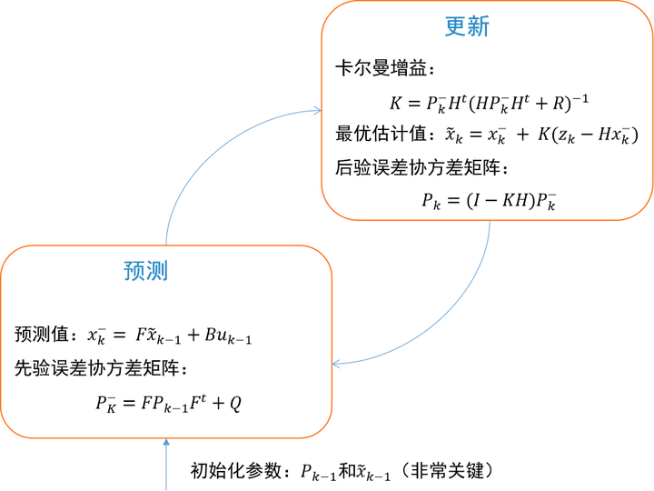
\includegraphics[width=0.78\textwidth]{assets/kalman_prediction_update_cycle.png}

\small
图：Kalman 预测--更新闭环总览。下文从后验误差方差最小化出发，依次推导图中的 Kalman 增益、后验均值与后验协方差。
\end{center}

\subsubsection*{1. Kalman 增益不是融合方差，而是由方差决定的最优融合权重}

先在一维直接测量 $H=1$ 的情况下完整推导。后验误差为
\begin{equation}
e_k=(1-K_k)e_k\prior-K_k\nu_k.
\end{equation}
先验误差与当前测量噪声不相关时，后验误差方差是
\begin{equation}
P_k(K_k)
=(1-K_k)^2P_k\prior+K_k^2R.
\end{equation}
为了寻找使后验方差最小的融合权重，对 $K_k$ 求导：
\begin{align}
\frac{\mathrm dP_k}{\mathrm dK_k}
&=\frac{\mathrm d}{\mathrm dK_k}
\left[(1-K_k)^2P_k\prior+K_k^2R\right]\\
&=-2(1-K_k)P_k\prior+2K_kR.
\end{align}
令导数为零：
\begin{align}
-2(1-K_k)P_k\prior+2K_kR&=0\\
(1-K_k)P_k\prior&=K_kR\\
P_k\prior-K_kP_k\prior&=K_kR\\
P_k\prior&=K_k(P_k\prior+R).
\end{align}
因此最优一维 Kalman 增益为
\begin{equation}
\boxed{
K_k=\frac{P_k\prior}{P_k\prior+R}
}.
\end{equation}
它是无量纲融合权重，而不是方差。把它代回方差公式，才得到融合后的后验方差：
\begin{equation}
\boxed{
P_k
=\frac{P_k\prior\!\cdot R}{P_k\prior+R}
=\left[(P_k\prior)^{-1}+R^{-1}\right]^{-1}
}.
\end{equation}

多维情况下仍然选择使后验总方差最小的 $K_k$。Joseph 形式在任意候选增益 $K_k$ 下为
\begin{equation}
P_k(K_k)
=(I-K_kH)P_k\prior(I-K_kH)\transpose+K_kRK_k\transpose.
\end{equation}
将其展开，并定义创新协方差
\begin{equation}
S_k=HP_k\prior H\transpose+R,
\end{equation}
得到
\begin{equation}
P_k(K_k)
=P_k\prior-K_kHP_k\prior
-P_k\prior H\transpose K_k\transpose
+K_kS_kK_k\transpose.
\end{equation}
用 $\operatorname{tr}(P_k)$ 表示各状态后验方差之和。由于 $P_k\prior$、$R$ 和 $S_k$ 都是对称矩阵，对 $K_k$ 求矩阵导数：
\begin{equation}
\frac{\partial\,\operatorname{tr}(P_k)}{\partial K_k}
=-2P_k\prior H\transpose+2K_kS_k.
\end{equation}
令该导数为零：
\begin{align}
-2P_k\prior H\transpose+2K_kS_k&=0\\
K_kS_k&=P_k\prior H\transpose\\
K_k&=P_k\prior H\transpose S_k^{-1}.
\end{align}
代回 $S_k$，得到图中的矩阵 Kalman 增益：
\begin{equation}
\boxed{
K_k
=P_k\prior H\transpose
(HP_k\prior H\transpose+R)^{-1}
}.
\end{equation}

\begin{keybox}
$K_k$ 的准确称呼是 Kalman 增益或最优融合权重。它由先验协方差 $P_k\prior$、测量映射 $H$ 和测量噪声协方差 $R$ 共同决定。真正表示高斯融合后分布宽度的是后验协方差 $P_k$。
\end{keybox}

\subsubsection*{2. 最优估计是先验状态估计加上“增益乘创新”}

预测阶段给出先验状态估计 $\hat{\bm x}_k\prior$。测量值与先验预测测量之间的差称为创新：
\begin{equation}
\bm r_k
=\bm z_k-H\hat{\bm x}_k\prior.
\end{equation}
最优后验状态估计为
\begin{equation}
\boxed{
\hat{\bm x}_k
=\hat{\bm x}_k\prior
+K_k(\bm z_k-H\hat{\bm x}_k\prior)
}.
\end{equation}
所以这里相加的是“先验状态估计”，不是“先验误差”。$K_k\bm r_k$ 是估计中心从先验均值移动到后验均值的修正量：
\begin{equation}
K_k\bm r_k
=\hat{\bm x}_k-\hat{\bm x}_k\prior.
\end{equation}

\subsubsection*{3. 后验分布与融合协方差}

完成测量更新后，状态的后验高斯分布为
\begin{equation}
\boxed{
\bm x_k\mid\bm z_{1:k}
\sim
\mathcal N(\hat{\bm x}_k,P_k)
}.
\end{equation}
程序使用数值稳定的 Joseph 形式计算融合协方差：
\begin{equation}
\boxed{
P_k
=(I-K_kH)P_k\prior(I-K_kH)\transpose
+K_kRK_k\transpose
}.
\end{equation}
在 $K_k$ 取最优 Kalman 增益时，它与下面两种高斯融合写法完全等价：
\begin{equation}
\boxed{
P_k
=(I-K_kH)P_k\prior
=\left[(P_k\prior)^{-1}+H\transpose R^{-1}H\right]^{-1}
}.
\end{equation}
一维直接测量时进一步化为
\begin{equation}
\boxed{
P_k
=\frac{P_k\prior\!\cdot R}{P_k\prior+R}
}.
\end{equation}
因此，$K_k$ 是融合权重，$P_k$ 才是先验高斯与测量高斯融合后的协方差。

\subsubsection*{4. 过程噪声协方差 \texorpdfstring{$Q_k$}{Qk} 怎样进入下一次先验}

后验状态经过运动模型传播，形成下一步先验均值：
\begin{equation}
\hat{\bm x}_{k+1}\prior
=F_k\hat{\bm x}_k+B_ku_k.
\end{equation}
对应的先验协方差为
\begin{equation}
\boxed{
P_{k+1}\prior
=F_kP_kF_k\transpose+Q_k
}.
\end{equation}
$F_kP_kF_k\transpose$ 是上一时刻后验不确定性经过载具运动学传播后的结果；$Q_k$ 是本次传播新增加的过程噪声协方差，用来描述加速度变化、打滑、执行器偏差和模型不完整性。

因此，下一时刻的先验协方差同时包含两部分：
\begin{equation}
\underbrace{P_{k+1}\prior}_{\text{下一时刻先验不确定性}}
=
\underbrace{F_kP_kF_k\transpose}_{\text{旧不确定性的运动传播}}
+
\underbrace{Q_k}_{\text{本次运动新增的不确定性}}.
\end{equation}
载具运动不会使 $P_k$ 简单恢复为 $Q_k$；更准确的说法是：载具运动将原有后验协方差通过 $F_k$ 传播，同时把 $Q_k$ 累加到下一时刻先验协方差中。

\subsubsection*{5. 预测状态分布、对角元素和 \texorpdfstring{$H$}{H} 的测量空间变换}

给定此前全部观测 $\bm z_{1:k-1}$，预测状态的联合先验分布为
\begin{equation}
\boxed{
\bm x_k\mid\bm z_{1:k-1}
\sim
\mathcal N(\hat{\bm x}_k\prior,P_k\prior)
}.
\end{equation}
这里必须使用完整矩阵 $P_k\prior$，因为其非对角元素保存了不同状态误差之间的关联。只有单独观察第 $i$ 个状态分量时，才写成边缘分布
\begin{equation}
x_{i,k}\mid\bm z_{1:k-1}
\sim
\mathcal N\!\left(
\hat x_{i,k}\prior,\,
(P_k\prior)_{ii}
\right).
\end{equation}
因此，对角元素 $(P_k\prior)_{ii}$ 是第 $i$ 个状态分量的预测方差；非对角元素不能在联合滤波中丢弃。

将预测状态映射到测量空间。先定义无噪声预测测量
\begin{equation}
\bm y_k=H\bm x_k.
\end{equation}
线性变换后的高斯分布为
\begin{equation}
\bm y_k\mid\bm z_{1:k-1}
\sim
\mathcal N\!\left(
H\hat{\bm x}_k\prior,\,
HP_k\prior H\transpose
\right).
\end{equation}
实际测量还包含 $\bm\nu_k\sim\mathcal N(0,R)$，所以
\begin{equation}
\boxed{
\bm z_k\mid\bm z_{1:k-1}
\sim
\mathcal N\!\left(
H\hat{\bm x}_k\prior,\,
HP_k\prior H\transpose+R
\right)
}.
\end{equation}
其中
\begin{equation}
S_k=HP_k\prior H\transpose+R
\end{equation}
就是创新协方差。对于本项目的状态 $[x,y,v]\transpose$ 和二维位置观测，
\begin{equation}
H=
\begin{bmatrix}
1&0&0\\
0&1&0
\end{bmatrix},
\end{equation}
因此
\begin{equation}
HP_k\prior H\transpose
=
\begin{bmatrix}
p_{xx}&p_{xy}\\
p_{xy}&p_{yy}
\end{bmatrix}.
\end{equation}
它不仅保留位置方差 $p_{xx},p_{yy}$，还保留位置误差之间的关联 $p_{xy}$。速度虽然不被直接测量，但 $P_k\prior H\transpose$ 中的 $p_{xv},p_{yv}$ 会使位置创新继续修正速度。

\begin{center}
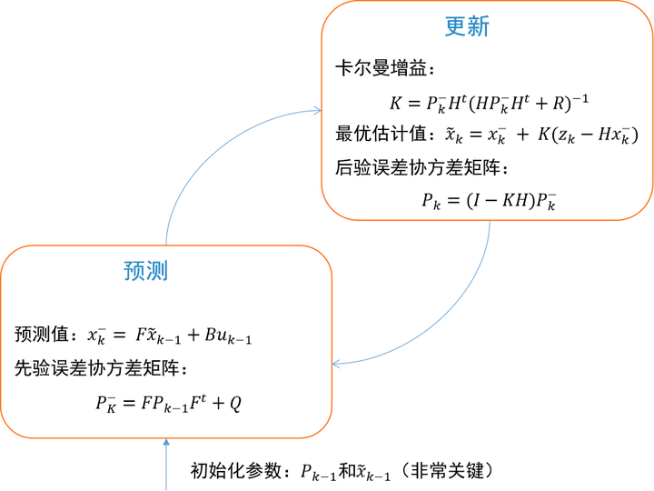
\includegraphics[width=0.88\textwidth]{assets/kalman_prediction_update_cycle.png}

\small
图：Kalman 预测--更新闭环。图中的
$P_k=(I-K_kH)P_k\prior$
是最优增益下的协方差简化式；本项目程序使用与其理论等价、数值更稳定的 Joseph 形式。
\end{center}

\section{协方差元素的来源、物理含义与 \texorpdfstring{$p_{xy}=0$}{pxy=0} 对照实验}

本节把前文最初介绍的“标准差如何组成协方差矩阵”和“多元高斯如何映射为向量与矩阵”合并到当前程序的运动传播中，再用实际数值说明非对角元素如何产生、如何进入 Kalman 增益，以及为什么在本项目的特定模型和参数下，强制令 $p_{xy}=0$ 反而可能减小位置误差。

\subsection{从标准差清单到联合高斯协方差矩阵}

若第 $i$ 个状态量的先验标准差为 $\sigma_i\prior$，标准差可以写成列向量
\begin{equation}
\bm\sigma_k\prior=
\begin{bmatrix}
\sigma_1\prior&\sigma_2\prior&\cdots&\sigma_n\prior
\end{bmatrix}\transpose,
\end{equation}
但它不是协方差矩阵。若各状态误差彼此独立，则
\begin{equation}
P_k\prior=\operatorname{diag}\!\left(
(\sigma_1\prior)^2,(\sigma_2\prior)^2,\ldots,(\sigma_n\prior)^2
\right).
\end{equation}
若状态误差之间有关联，则一般元素为
\begin{equation}
(P_k\prior)_{ij}
=\operatorname{Cov}(e_{i,k}\prior,e_{j,k}\prior)
=\rho_{ij}\sigma_i\prior\sigma_j\prior,
\qquad \rho_{ii}=1.
\end{equation}

对本项目的状态
\begin{equation}
\bm x_k=
\begin{bmatrix}x_k&y_k&v_k\end{bmatrix}\transpose,
\end{equation}
测量到来之前的联合先验分布写成
\begin{equation}
\bm x_k\mid\bm z_{1:k-1}
\sim\mathcal N(\hat{\bm x}_k\prior,P_k\prior),
\end{equation}
其中
\begin{equation}
P_k\prior=
\begin{bmatrix}
p_{xx}&p_{xy}&p_{xv}\\
p_{xy}&p_{yy}&p_{yv}\\
p_{xv}&p_{yv}&p_{vv}
\end{bmatrix}.
\end{equation}
对角元素是各状态误差的方差；非对角元素是不同状态误差之间的协方差。特别地，$p_{xv}$ 和 $p_{yv}$ 是位置创新修正速度的直接通道，而 $p_{xy}$ 描述 $x$、$y$ 两个位置误差应当如何联合解释。

\subsection{为什么协方差矩阵必然对称}

协方差满足
\begin{align}
\operatorname{Cov}(e_i,e_j)
&=\mathbb E[(e_i-\mathbb E[e_i])(e_j-\mathbb E[e_j])]\\
&=\mathbb E[(e_j-\mathbb E[e_j])(e_i-\mathbb E[e_i])]\\
&=\operatorname{Cov}(e_j,e_i),
\end{align}
因为两个标量相乘时交换顺序不会改变结果。因此
\begin{equation}
\boxed{p_{xy}=p_{yx},\qquad p_{xv}=p_{vx},\qquad p_{yv}=p_{vy}},
\end{equation}
也即 $P_k\prior=(P_k\prior)\transpose$。$p_{xy}$ 与 $p_{yx}$ 不是两个独立参数，而是同一个误差关联在矩阵中的对称位置。

\subsection{状态更新方程怎样产生 \texorpdfstring{$p_{xv}$、$p_{yv}$ 和 $p_{xy}$}{pxv, pyv and pxy}}

当前程序给定航向角 $\theta_k$、角速度 $w_k$ 和传播时间 $\Delta t$，先计算单位纵向速度在一个时间区间内造成的位移系数
\begin{equation}
a_k=
\begin{cases}
\dfrac{\sin(\theta_k+w_k\Delta t)-\sin\theta_k}{w_k},&|w_k|>0,\\[1.1ex]
\cos\theta_k\,\Delta t,&w_k=0,
\end{cases}
\end{equation}
\begin{equation}
b_k=
\begin{cases}
\dfrac{\cos\theta_k-\cos(\theta_k+w_k\Delta t)}{w_k},&|w_k|>0,\\[1.1ex]
\sin\theta_k\,\Delta t,&w_k=0.
\end{cases}
\end{equation}
它们不是额外调参系数，而是由载具的同构圆弧运动学和状态更新时间尺度共同确定的。状态传播及其局部线性矩阵为
\begin{equation}
\hat{\bm x}_{k+1}\prior=
\begin{bmatrix}
\hat x_k+a_k\hat v_k\\
\hat y_k+b_k\hat v_k\\
\hat v_k
\end{bmatrix},
\qquad
F_k=
\begin{bmatrix}
1&0&a_k\\
0&1&b_k\\
0&0&1
\end{bmatrix}.
\end{equation}

先从一个对角后验协方差开始：
\begin{equation}
P_k=
\begin{bmatrix}
p_{xx}&0&0\\
0&p_{yy}&0\\
0&0&p_{vv}
\end{bmatrix}.
\end{equation}
完整执行矩阵乘法，先有
\begin{equation}
F_kP_k=
\begin{bmatrix}
p_{xx}&0&a_kp_{vv}\\
0&p_{yy}&b_kp_{vv}\\
0&0&p_{vv}
\end{bmatrix},
\end{equation}
再右乘 $F_k\transpose$：
\begin{equation}
F_kP_kF_k\transpose=
\begin{bmatrix}
p_{xx}+a_k^2p_{vv}&a_kb_kp_{vv}&a_kp_{vv}\\
a_kb_kp_{vv}&p_{yy}+b_k^2p_{vv}&b_kp_{vv}\\
a_kp_{vv}&b_kp_{vv}&p_{vv}
\end{bmatrix}.
\end{equation}
最后再加入过程噪声协方差 $Q_k$：
\begin{equation}
P_{k+1}\prior=F_kP_kF_k\transpose+Q_k.
\end{equation}
因此，即使初始非对角元素全部为零，运动传播后也会自然产生
\begin{equation}
p_{xv}\prior\approx a_kp_{vv},\qquad
p_{yv}\prior\approx b_kp_{vv},\qquad
p_{xy}\prior\approx a_kb_kp_{vv},
\end{equation}
其中“$\approx$”表示暂时只突出 $p_{vv}$ 经运动传播产生的主要项，尚未把原有非对角元素和 $Q_k$ 的对应元素写入。

以程序初始化的 $p_{vv}=25$、$\Delta t=0.01\,\mathrm{s}$ 为例。若这一小段运动近似沿 $x$ 轴，$\theta_k\approx0$ 且 $w_k\approx0$，则
\begin{equation}
a_k\approx0.01,\qquad b_k\approx0.
\end{equation}
于是一次传播便给出
\begin{equation}
p_{xv}:0\longrightarrow a_kp_{vv}\approx0.01\times25=0.25,
\end{equation}
程序浮点结果约为 $0.249999$。这个数值不仅是矩阵运算结果，也有直接的物理含义：滤波器根据当前运动模型认为载具整体主要沿 $x$ 轴方向移动，因此“纵向速度估计偏大或偏小”会主要伴随“$x$ 位置预测偏大或偏小”，从而建立了 $x$ 位置误差与速度误差之间的关联。此时 $b_k\approx0$，所以 $p_{yv}$ 和由这一项产生的 $p_{xy}$ 仍接近零。

当载具斜向运动或转弯时，$a_k$、$b_k$ 同时非零，同一个速度误差会同时传播到 $x$、$y$ 两个方向，于是 $p_{xv}$、$p_{yv}$ 和 $p_{xy}$ 都会出现。非对角元素不是额外状态，也不是人为加入的模糊量，而是联合状态经过运动模型传播后形成的误差关联。

\subsection{三个交叉协方差怎样进入 Kalman 增益}

二维位置测量对应
\begin{equation}
H=
\begin{bmatrix}
1&0&0\\
0&1&0
\end{bmatrix},
\qquad
R=
\begin{bmatrix}
r_x&0\\
0&r_y
\end{bmatrix}.
\end{equation}
创新协方差为
\begin{equation}
S=HP\prior H\transpose+R
=
\begin{bmatrix}
p_{xx}+r_x&p_{xy}\\
p_{xy}&p_{yy}+r_y
\end{bmatrix}.
\end{equation}
定义
\begin{equation}
D=(p_{xx}+r_x)(p_{yy}+r_y)-p_{xy}^2,
\end{equation}
则
\begin{equation}
S^{-1}=\frac{1}{D}
\begin{bmatrix}
p_{yy}+r_y&-p_{xy}\\
-p_{xy}&p_{xx}+r_x
\end{bmatrix}.
\end{equation}
状态--测量交叉协方差为
\begin{equation}
P\prior H\transpose=
\begin{bmatrix}
p_{xx}&p_{xy}\\
p_{xy}&p_{yy}\\
p_{xv}&p_{yv}
\end{bmatrix}.
\end{equation}
因此速度对应的第三行 Kalman 增益为
\begin{equation}
\begin{bmatrix}k_{vx}&k_{vy}\end{bmatrix}
=\begin{bmatrix}p_{xv}&p_{yv}\end{bmatrix}S^{-1},
\end{equation}
完全展开得到
\begin{equation}
\boxed{
k_{vx}
=\frac{p_{xv}(p_{yy}+r_y)-p_{yv}p_{xy}}{D}
},
\end{equation}
\begin{equation}
\boxed{
k_{vy}
=\frac{p_{yv}(p_{xx}+r_x)-p_{xv}p_{xy}}{D}
}.
\end{equation}

\begin{keybox}
$p_{xv}$、$p_{yv}$ 决定位置残差能否修正速度；$p_{xy}$ 决定两个位置残差应当如何联合解释。也就是说，$p_{xy}$ 不是“位置修正速度”的直接通道，但它通过 $S^{-1}$ 中的耦合项调整 $p_{xv}$、$p_{yv}$ 对两个位置创新的使用方式。
\end{keybox}

这类融合项在观测方向耦合明显、观测模型不确定或不同信息源需要联合解释时很有价值：交叉协方差使增益能够根据误差关联重新分配各观测分量的修正作用。但如果系统结构简单、$x$ 与 $y$ 的观测噪声实际独立，而模型产生的 $p_{xy}$ 不能准确代表真实误差关联，那么该耦合项也可能把一个方向的噪声带入另一个方向。此时令 $p_{xy}=0$ 相当于采用结构化协方差近似，使观测器更接近彼此独立的 $x$、$y$ 状态更新通道。

\subsection{航向角和角速度误差的边界}

当前滤波状态仅为 $[x,y,v]\transpose$；$\theta_k$ 与 $w_k$ 作为已知外部运动学输入直接进入 $a_k,b_k$，不进入 Kalman 状态和协方差。在仿真中二者来自真实领导者，因此这一假设成立。真实车辆中若使用
\begin{equation}
\widetilde\theta_k=\theta_k+n_{\theta,k},
\qquad
\widetilde w_k=w_k+n_{w,k},
\end{equation}
即使圆弧公式本身正确，错误的航向和角速度仍会通过 $a_k,b_k$ 造成位置预测误差，并使交叉协方差不能完全反映真实关联。

本项目暂不把 $\theta,w$ 加入当前位置 Kalman 状态，以避免角度估计超调直接影响编队控制。进入真实车辆实验后，可以把这部分不确定性折算进较大的 $Q_k$，或为航向与角速度设置独立估计器。换言之，融合项能够依据已有协方差修正增益，但不能替代对未知输入不确定性的建模。

\subsection{强制 \texorpdfstring{$p_{xy}=0$}{pxy=0} 的数值对照实验}

为检验上述耦合在当前具体模型中究竟有益还是有害，保留原程序不变，并复制一份对照程序，在每次预测和更新后都强制
\begin{equation}
p_{xy}=p_{yx}=0.
\end{equation}
两版程序使用相同随机种子、噪声序列、参数、$20\,\mathrm{s}$ 仿真时长和 $2001$ 个时间点。实验结果如下。

\begin{center}
\begin{tabularx}{0.96\textwidth}{Xrrr}
\toprule
指标 & 完整协方差 & 强制 $p_{xy}=0$ & 相对变化\\
\midrule
先验 $x$ RMSE & $0.026463\,\mathrm m$ & $0.017308\,\mathrm m$ & 降低 $34.59\%$\\
先验 $y$ RMSE & $0.020174\,\mathrm m$ & $0.018400\,\mathrm m$ & 降低 $8.79\%$\\
先验位置 RMSE & $0.033276\,\mathrm m$ & $0.025262\,\mathrm m$ & 降低 $24.08\%$\\
后验位置 RMSE & $0.031789\,\mathrm m$ & $0.023382\,\mathrm m$ & 降低 $26.44\%$\\
先验最大位置误差 & $0.186626\,\mathrm m$ & $0.186626\,\mathrm m$ & 相同\\
\bottomrule
\end{tabularx}
\end{center}

\begin{figure}[htbp]
\centering
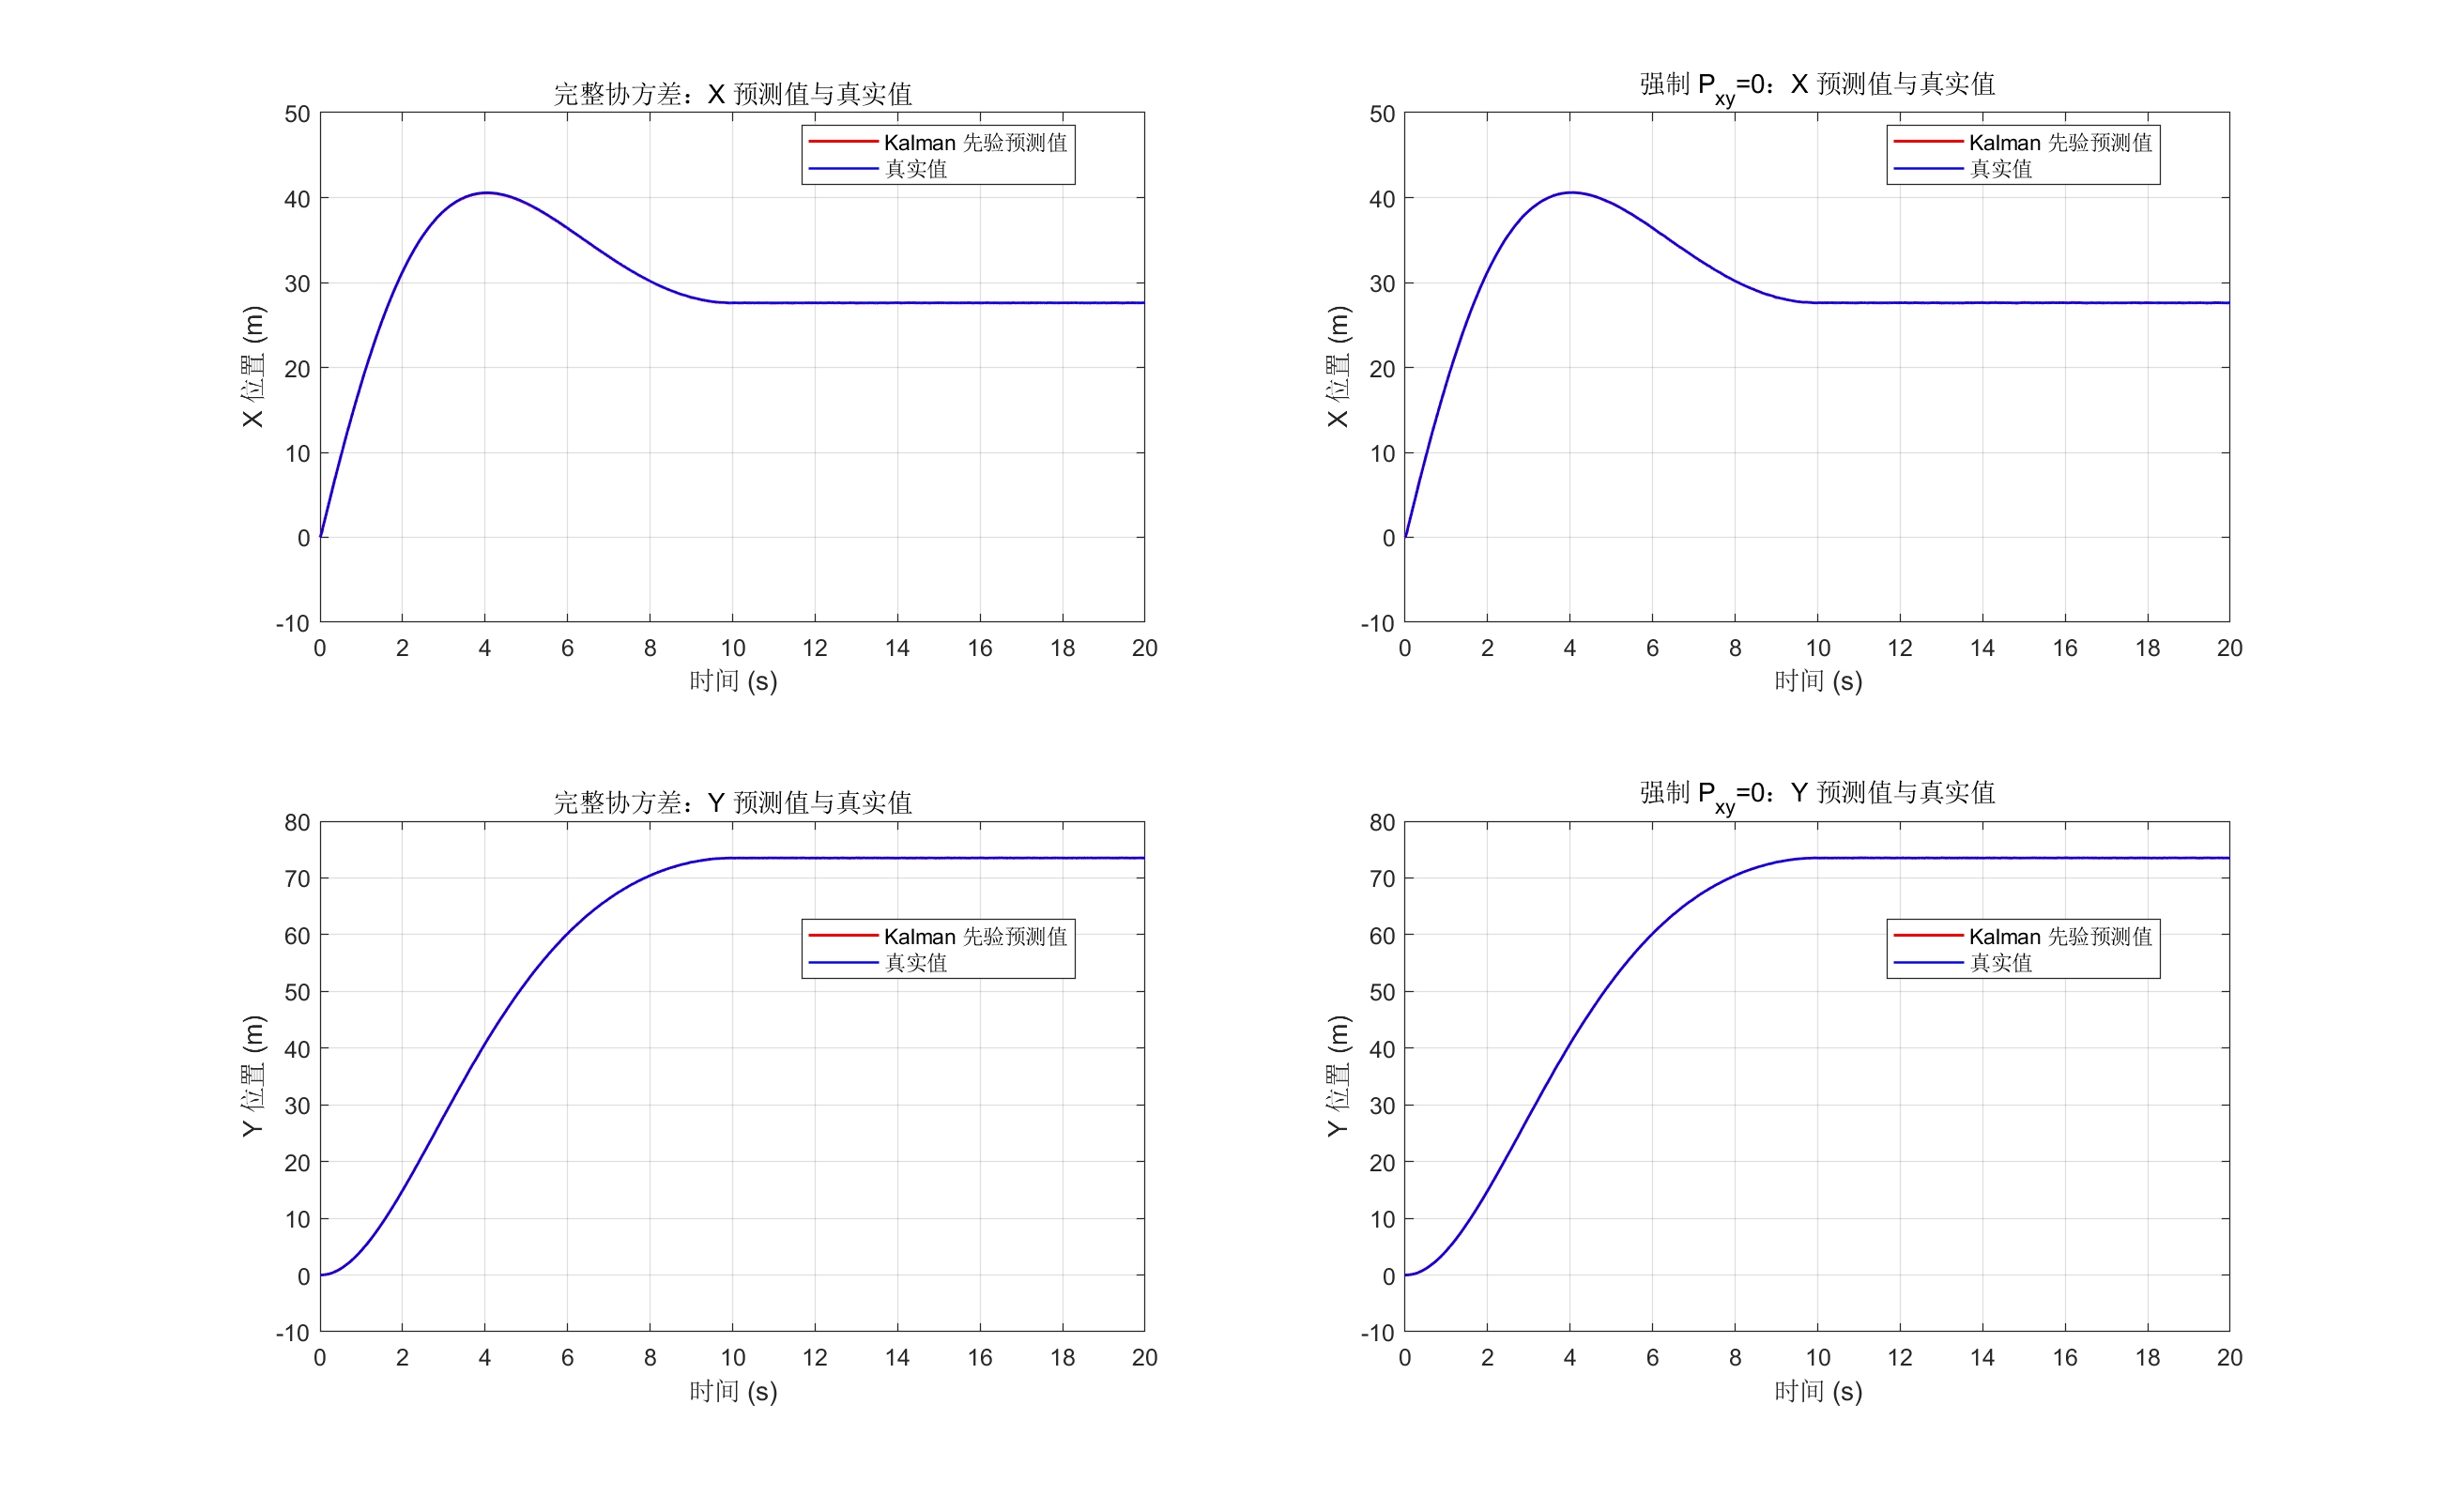
\includegraphics[width=0.96\textwidth]{../saves/kalman-pxy-prediction-vs-truth-26-11-16-183327.png}
\caption{完整协方差与强制 $p_{xy}=0$ 两种模型的 Kalman 先验预测值（红色）和真实值（蓝色）随时间的对比。}
\end{figure}

\begin{figure}[htbp]
\centering
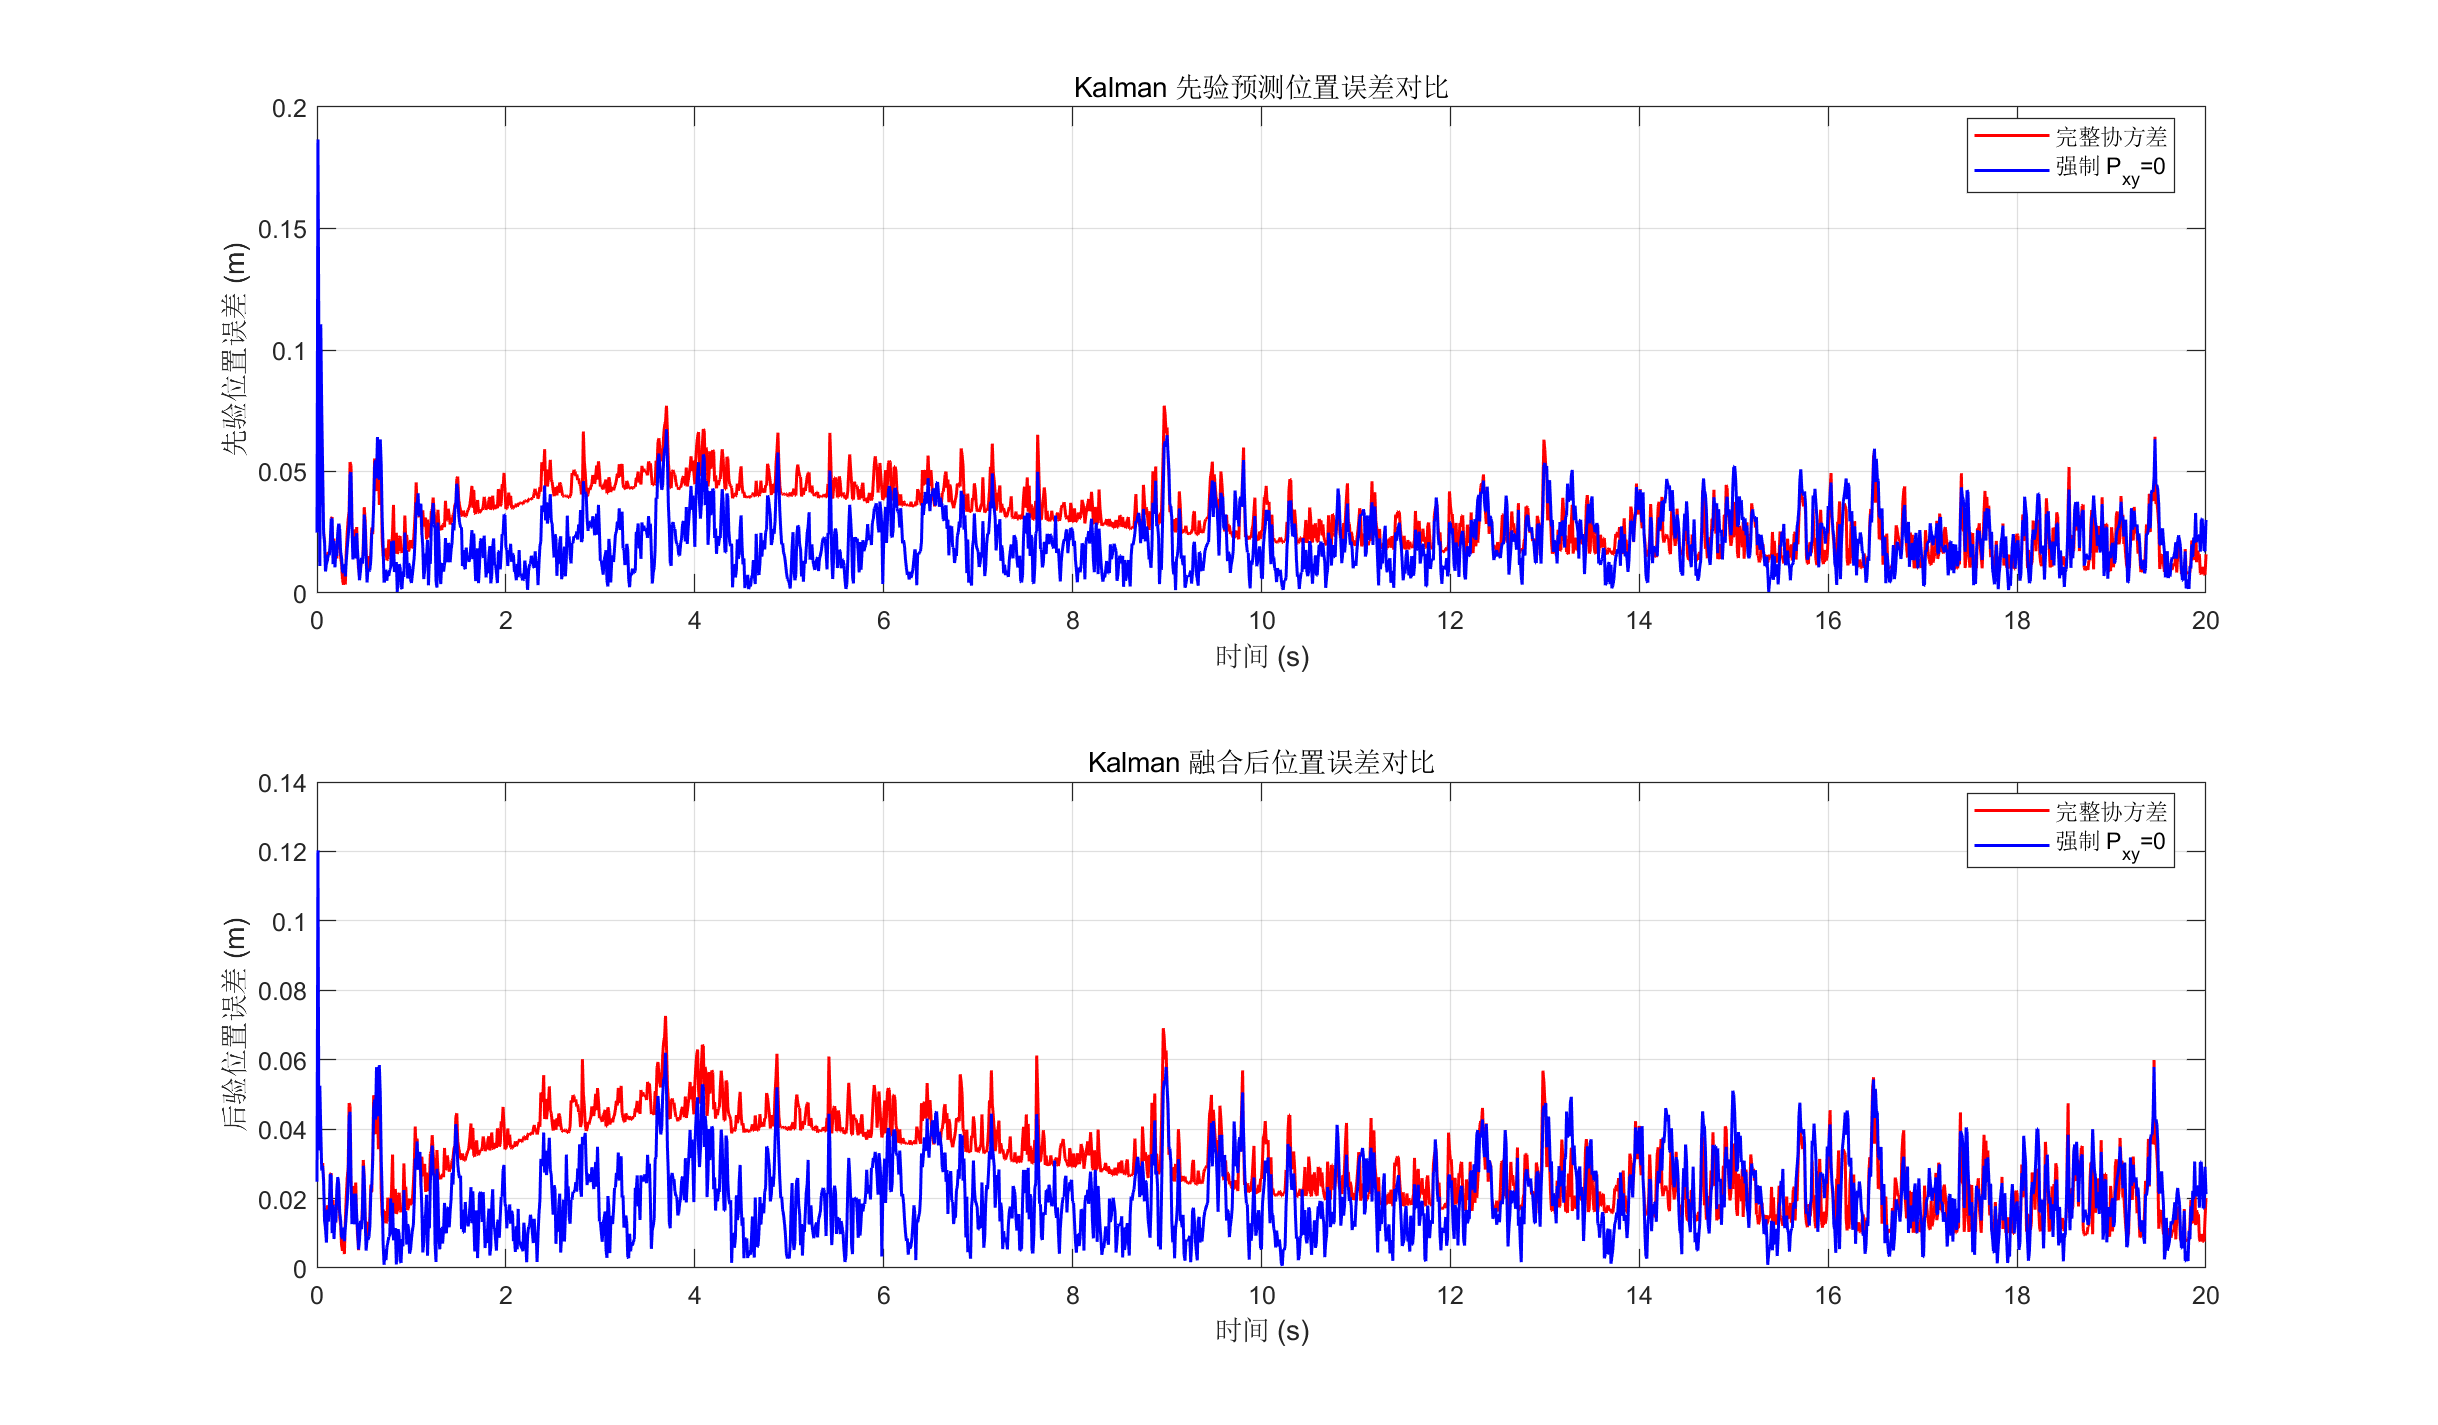
\includegraphics[width=0.96\textwidth]{../saves/kalman-pxy-error-comparison-26-11-16-183327.png}
\caption{位置预测误差随时间的对比：红色为完整协方差模型，蓝色为强制 $p_{xy}=0$ 的结构化协方差模型。}
\end{figure}

实验还核对了：对照版先验与后验 $p_{xy}$ 的最大绝对值均为零；原版先验 $|p_{xy}|$ 最大约为 $7.99\times10^{-4}$。因此，在这一次固定随机种子的实验中，强制 $p_{xy}=0$ 确实取得了更小的位置预测误差。这支持如下针对当前程序的解释：对于结构明确、位置观测噪声按 $x,y$ 独立建模的控制系统，不准确或不必要的交叉耦合可能传播噪声；把观测器结构直接约束为 $p_{xy}=0$，反而更贴近当前状态更新模型。

但是，这一结果只来自一条轨迹、一个随机种子和当前一组 $Q,R$ 参数，不能推出“任何 Kalman 滤波都应删除 $p_{xy}$”。$p_{xy}$ 在一般联合高斯模型中仍有严格的概率含义；是否将其清零，应视为一个需要多随机种子、不同转弯强度和不同噪声条件继续验证的结构化建模选择。

\clearpage
\section{与当前 MATLAB 实现的对应关系}

当前实现中的关键尺寸为
\begin{equation}
P_k\prior\in\mathbb R^{3\times3},\quad
H\in\mathbb R^{2\times3},\quad
R\in\mathbb R^{2\times2},\quad
S_k\in\mathbb R^{2\times2},\quad
K_k\in\mathbb R^{3\times2}.
\end{equation}

代码中的二维观测只包含 $x,y$；$v$ 通过 $P_k\prior$ 的第三行交叉协方差得到递归修正；$\theta,w$ 是运动学输入，不进入该 Kalman 状态。兼容字段 \texttt{state\_x/state\_y} 只是动画读取视图，真正递推的是三维 \texttt{state} 和 $3\times3$ 的 \texttt{covariance}。

主要程序变量与数学符号逐项对应如下：
\begin{center}
\begin{tabularx}{0.96\textwidth}{>{\ttfamily\small}p{48mm}>{\centering\arraybackslash}p{22mm}X}
\toprule
\normalfont 程序变量 & 数学符号 & 内容\\
\midrule
previous\_posterior\_state & $\hat{\bm x}_{k-1}$ & 上一时刻后验均值\\
previous\_posterior\_\newline covariance & $P_{k-1}$ & 上一时刻后验协方差\\
prior\_state & $\hat{\bm x}_k\prior$ & 当前预测均值\\
prior\_covariance & $P_k\prior$ & 当前先验误差协方差\\
position\_observation & $\bm z_k$ & 当前二维带噪声位置观测\\
observation\_covariance & $R$ & 测量噪声协方差\\
innovation & $\bm r_k$ & 测量减去预测测量\\
innovation\_covariance & $S_k$ & 创新的协方差，不是后验协方差\\
kalman\_gain & $K_k$ & 把创新映射为状态均值修正量\\
posterior\_state & $\hat{\bm x}_k$ & 融合后的后验均值\\
posterior\_covariance & $P_k$ & 融合后的后验误差协方差\\
\bottomrule
\end{tabularx}
\end{center}

因此代码中的三条关键计算应按下面的语义阅读：
\begin{align}
\texttt{innovation}
&\longleftrightarrow \bm z_k-H\hat{\bm x}_k\prior,\\
\texttt{kalman\_gain * innovation}
&\longleftrightarrow K_k\bm r_k
=\hat{\bm x}_k-\hat{\bm x}_k\prior,\\
\texttt{posterior\_covariance}
&\longleftrightarrow
(I-K_kH)P_k\prior(I-K_kH)\transpose+K_kRK_k\transpose.
\end{align}

第二行明确表示均值的修正量；第三行才表示融合后误差分布的宽度和状态间剩余关联。

\clearpage
\subsection{递推过程与编队跟踪结果的综合可视化}

图~\ref{fig:kalman-prediction-visualbility} 给出了强制 $p_{xy}=0$ 的结构化协方差版本在 $t=20\,\mathrm{s}$ 时的综合画面。左侧展示真实领导者与四个跟随者的完整运动轨迹，并额外标出仅用于观察、而不参与控制的 $0.1\,\mathrm{s}$ 预测领导者。右上把位置先验分布、带噪声观测分布和融合后验分布叠加到同一个 $x$--$y$--概率密度坐标系中，使“两个信息来源如何形成后验分布”可以直接观察。右中对照速度先验、由后验位置窗口推导的速度信息与现有 Kalman 速度后验；右下则给出后验位置相对真实位置的误差模值随时间的变化。

这张图把前文的三条主线放到同一时刻下核对：位置高斯分布的矩阵融合产生后验状态；后验位置与运动模型共同约束速度估计；最终状态估计再服务于编队跟踪。图中的预测领导者只承担可视化比较作用，控制算法仍使用当前后验领导者，因而不会把 $0.1\,\mathrm{s}$ 前视量误当成当前控制目标。

\begin{figure}[htbp]
\centering
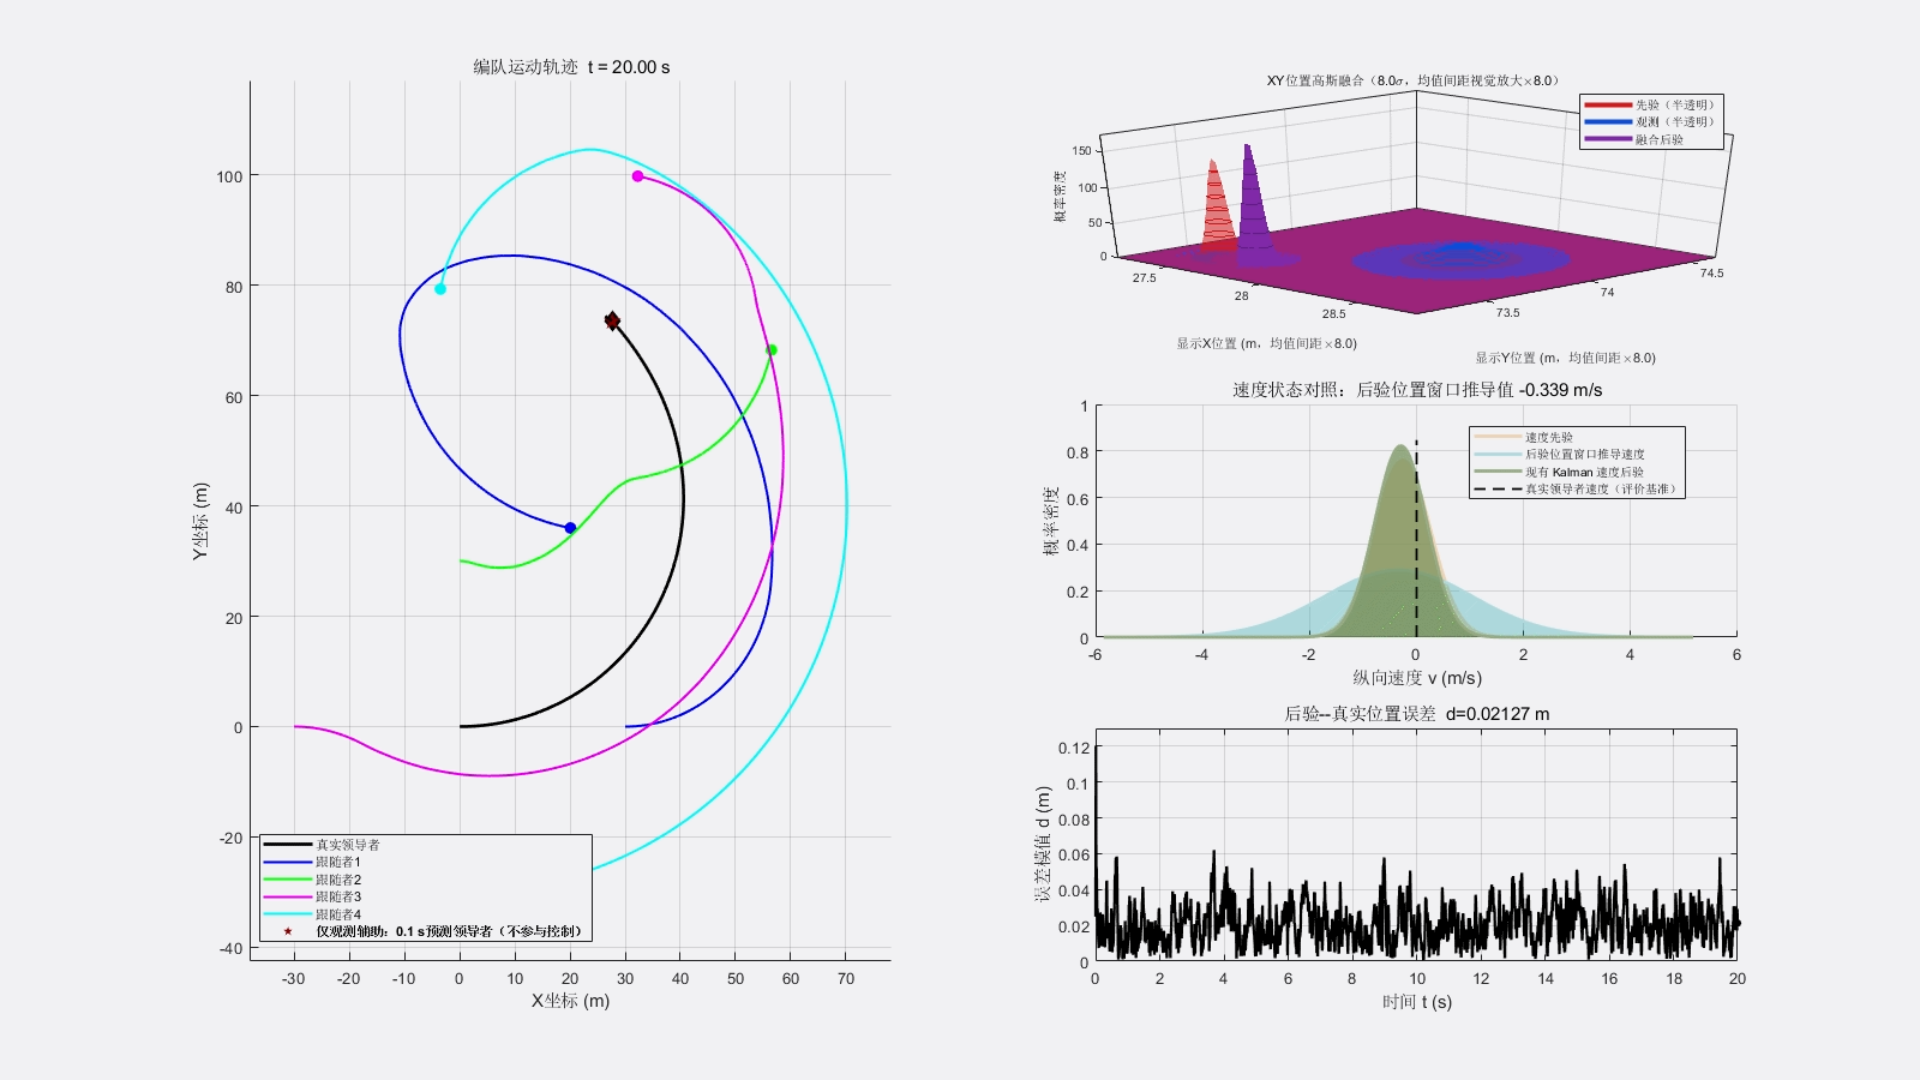
\includegraphics[width=0.99\textwidth]{assets/kalman-prediction-visualbility.png}
\caption{Kalman 预测虚拟领导者算法的综合可视化结果：左侧为编队运动轨迹；右上为位置先验、观测和后验高斯分布的三维叠加；右中为速度概率分布对照；右下为后验位置误差模值随时间的变化。}
\label{fig:kalman-prediction-visualbility}
\end{figure}

\end{document}
